\documentclass[11pt]{article}

\usepackage[T1]{fontenc}
\usepackage[utf8]{inputenc}
\usepackage{lmodern}
\usepackage[margin=1in]{geometry}
\usepackage{amsmath}
\usepackage{amssymb}
\usepackage{amsthm}
\usepackage{array}
\usepackage{bbm}
\usepackage{booktabs}
\usepackage[labelfont=bf]{caption}
\usepackage{float}
\usepackage{graphicx}
\usepackage{hyperref}
\usepackage{longtable}
\usepackage{makecell}
\usepackage{multirow}
\usepackage[round,authoryear]{natbib}
\usepackage{url}

\graphicspath{{build/figures/}}
\hypersetup{
  colorlinks = true,
  linkcolor = blue,
  citecolor = blue,
  urlcolor = blue
}

\setlength{\parindent}{0pt}
\setlength{\parskip}{0.75em}
\setlength{\emergencystretch}{2em}
\hfuzz=3pt
\hbadness=10000
\allowdisplaybreaks

\DeclareMathOperator*{\E}{E}
\DeclareMathOperator*{\logit}{logit}
\DeclareMathOperator*{\Bernoulli}{Bernoulli}
\DeclareMathOperator*{\Beta}{Beta}

\newtheorem{proposition}{Proposition}
\newtheorem{lemma}[proposition]{Lemma}

\input{build/generated-values.tex}

\title{Testing two-component treatment effects in truncated continuous outcomes}
\author{
  Andreas Kryger Jensen and Theis Lange\\
  Section of Biostatistics, Department of Public Health\\
  University of Copenhagen
}
\date{}

\begin{document}

\maketitle

\begin{abstract}
Continuous outcomes such as quality-of-life scores are often undefined after death or a related event. A common pragmatic solution is to encode such patients by the worst possible score and analyze the resulting composite outcome with a one-dimensional procedure. That preserves a clinically meaningful ordering, but it conflates treatment effects on the atom with treatment effects on the continuous part among those with observed outcomes. We propose likelihood-ratio tests for the joint null of no treatment effect on either component. The construction yields a single prespecified p-value together with interpretable component-wise effect estimates and confidence regions. We present both a parametric version and a semi-parametric version based on empirical likelihood, establish their large-sample calibration, and study their behavior in simulations. The methods are most advantageous when component effects can be obscured by the one-dimensional composite or when survivor-distribution features make standard combined-outcome tests inefficient. A clinical application to the IST-3 acute ischemic stroke trial illustrates the method using death by six months as the atom and EuroQol visual analogue score among survivors as the continuous component.
\end{abstract}

\begin{center}
\textbf{Keywords:} Quality of Life, Randomized Controlled Trials,\\
Truncated Outcomes, Semi-Continuous Distributions, Empirical Likelihood
\end{center}

\section{Introduction}

Continuous outcomes such as quality-of-life scores, cognition scores, and days alive outside hospital are increasingly used in randomized trials of serious illness. When patients die before assessment, however, those outcomes are undefined rather than merely missing, creating the truncation-by-death problem \citep{Frangakis_2002,Colantuoni_2018}. Composite outcomes that combine mortality with an otherwise continuous scale are common in critical care and related areas; familiar examples include ventilator-free days and days alive without life support \citep{10.1001/jama.2021.18295,Yehya_2019}.

One pragmatic response is to place death, or another substantively distinct event, at the bottom of a single ordered scale and analyze the resulting composite with a rank-based or related one-dimensional method. Worst-rank analyses and related composite rankings have been advocated precisely because they retain all randomized patients in the primary analysis \citep{Lachin_1999,McMahon_2000,Colantuoni_2018}. The same logic underlies the widespread use of atom-at-zero outcomes such as ventilator-free days, where death is assigned the worst possible value on the scale \citep{Yehya_2019}. Throughout, we refer to the Mann--Whitney--Wilcoxon rank-sum test simply as the Wilcoxon test \citep{wilcoxon3001968individual,mann1947test}.

That strategy is often clinically sensible, but it targets the distribution of the composite outcome itself. It does not separate treatment effects on the probability of the atom from treatment effects on the continuous outcome among patients with observed values. When the two components move in different directions, or when treatment acts mainly through one of them, a one-dimensional analysis can be attenuated because opposite component effects partially cancel on the combined scale. The issue is therefore not only one of robustness or convenience; it is also one of estimand alignment.

Other approaches address truncated-by-death outcomes from different perspectives. Survivor-only analyses condition on a post-randomization event and therefore answer a conditional question that can differ materially from the intention-to-treat comparison. Principal-stratification and survivor-average-causal-effect approaches instead target causal effects in latent survivor strata, but they require assumptions that are not identified from the observed trial data alone \citep{Frangakis_2002,Colantuoni_2018}. Composite-endpoint approaches avoid that latent-stratum target by working directly with an ordered endpoint, but then the estimand is tied to the chosen ranking \citep{McMahon_2000,Colantuoni_2018}. Our goal in this paper is narrower and more operational: we target the joint observed-data null of no treatment effect on the atom probability and no treatment effect on the continuous component among those for whom it is observed.

Our construction combines ideas from two-part models for semi-continuous outcomes \citep{aitchison1955distribution,cragg1971some} and empirical-likelihood inference for mean restrictions \citep{owen1988empirical,owen1991empirical,kitamura2001asymptotic}. We develop a factorized likelihood-ratio framework that yields a single prespecified p-value for the joint null together with interpretable component-wise effect estimates and confidence regions. We present both a parametric version, which is efficient under a credible model for the non-atom component, and a semi-parametric version, which relaxes that distributional commitment while retaining the same Bernoulli component. The resulting procedures preserve the clinically meaningful atom used in practice, but they test a sharper question than direct one-dimensional analyses of the combined outcome.

Although we motivate the method by quality of life truncated by death, the same structure arises whenever one special value has a substantively different meaning than the remainder of an otherwise continuous scale. The target is an observed-data treatment contrast, not a principal-stratum causal estimand. The rest of the paper is organized as follows. Section~\ref{sec:method} introduces the statistical setup and the proposed tests. Section~\ref{sec:simulation-study} reports a simulation study, Section~\ref{sec:application} gives a clinical application, and Section~\ref{sec:discussion} concludes. Additional simulation results are collected in Appendix~\ref{app:supplementary-simulation-results}.

\section{Method}\label{sec:method}


Let data be independent and identically distributed random variables $(Y_i, A_i, R_i, X_i)$ for $i = 1, \ldots, n$, where $Y_i$ is a continuous outcome when it is defined, $A_i \in \{0,1\}$ indicates whether the outcome is defined and observed, $R_i \in \{0,1\}$ is the treatment indicator, and $X_i$ is a $p$-dimensional vector of baseline covariates. Because $Y_i$ is only meaningful when $A_i = 1$, we define the null hypothesis of no treatment effect as the joint equality
\begin{align*}
  \mathcal{L}(Y_i \mid A_i = 1, R_i = 1, X_i)
  &= \mathcal{L}(Y_i \mid A_i = 1, R_i = 0, X_i),\\
  \Pr(A_i = 1 \mid R_i = 1, X_i)
  &= \Pr(A_i = 1 \mid R_i = 0, X_i).
\end{align*}
In practice, this bivariate object is often replaced by a single combined outcome. Let $\mathcal{Y}\subseteq\mathbb{R}$ be the support of the non-atom outcome $Y_i\mid A_i=1$, and let $\mathcal{E}\notin\mathcal{Y}$ be a distinguished symbol representing the atom event. Define
\begin{align}
  \widetilde{\mathcal{Y}}
  &=
  \mathcal{Y}\sqcup\{\mathcal{E}\},\nonumber\\
  \widetilde{Y}_i
  &=
  \begin{cases}
    Y_i, & A_i=1,\\
    \mathcal{E}, & A_i=0.
  \end{cases}\label{eq:combinedOutcome}
\end{align}
where $\sqcup$ denotes disjoint union. Thus $\mathcal{E}$ is an abstract atom, not a real number, and is distinct from every ordinary non-atom outcome. We equip $\widetilde{\mathcal{Y}}$ with the $\sigma$-algebra
\[
  \widetilde{\mathcal{B}} = \{B,\; B \cup \{\mathcal{E}\} : B \in \mathcal{B}(\mathcal{Y})\},
\]
where $\mathcal{B}(\mathcal{Y})$ is the Borel $\sigma$-algebra on $\mathcal{Y}$ induced by $\mathbb{R}$.

For a chosen numerical code $e_0\in\mathbb{R}$, define
\[
  c_{e_0}:\widetilde{\mathcal{Y}}\to\mathbb{R},
  \qquad
  c_{e_0}(y)=y \quad (y\in\mathcal{Y}),
  \qquad
  c_{e_0}(\mathcal{E})=e_0,
\]
and write
\[
  \widetilde{Y}_i^{(e_0)}
  =c_{e_0}(\widetilde{Y}_i)
  =A_iY_i+(1-A_i)e_0.
\]
Arithmetic summaries are taken on $\widetilde{Y}_i^{(e_0)}$, not on the abstract atom $\mathcal{E}$. If $e_0\notin\mathcal{Y}$, the map $c_{e_0}$ is an injective numerical representation of the disjoint-union outcome. If $e_0\in\mathcal{Y}$, the coded value $\widetilde{Y}_i^{(e_0)}=e_0$ does not by itself identify the atom event; the distinction is retained through $A_i$ or, equivalently, through the abstract value $\widetilde{Y}_i=\mathcal{E}$. The distribution of $\widetilde{Y}_i$ is therefore a mixture of a point mass at $\mathcal{E}$ and a non-atom distribution on the support of $Y_i \mid A_i = 1$.

For $r\in\{0,1\}$, write
\[
  \pi_r(x)=\Pr(A_i=1\mid R_i=r,X_i=x),
  \qquad
  \mu_r(x)=\E(Y_i\mid A_i=1,R_i=r,X_i=x).
\]
The conditional mean of the coded numerical outcome is
\[
  \E\{\widetilde{Y}_i^{(e_0)}\mid R_i=r,X_i=x\}
  = e_0\{1-\pi_r(x)\}+\pi_r(x)\mu_r(x).
\]
This quantity can be identical between treatment groups even when treatment affects both the observation probability and the continuous component. To see this, let
\[
  \mu_0(x)=\mu(x),
  \qquad
  \mu_1(x)=\mu(x)+\mu_\delta(x).
\]
Then
\begin{align}
  \Delta_{\widetilde{Y}}^{(e_0)}(x)
  &= \E\{\widetilde{Y}_i^{(e_0)}\mid R_i=1,X_i=x\}
     -\E\{\widetilde{Y}_i^{(e_0)}\mid R_i=0,X_i=x\}\nonumber\\
  &= e_0\{\pi_0(x)-\pi_1(x)\}
     +\pi_1(x)\mu_1(x)-\pi_0(x)\mu_0(x)\label{eq:Delta}\\
  &= \{\mu(x)-e_0\}\{\pi_1(x)-\pi_0(x)\}
     +\pi_1(x)\mu_\delta(x).\nonumber
\end{align}
Here $\Delta_{\widetilde{Y}}^{(e_0)}(x)$ is a contrast on the coded numerical representation $\widetilde{Y}_i^{(e_0)}$, not a mean on the abstract disjoint-union space.
Choosing
\[
  \mu_\delta(x)
  =\{\mu(x)-e_0\}
  \left\{\frac{\pi_0(x)}{\pi_1(x)}-1\right\}
\]
forces $\Delta_{\widetilde{Y}}^{(e_0)}(x)=0$ even though both components depend on treatment. For $e_0=0$, this reduces to the atom-at-zero formula. Thus testing $\Delta_{\widetilde{Y}}^{(e_0)}(x)=0$ is generally not equivalent to testing no treatment effect on the joint observed-data structure, and the latter requires two restrictions.

The event $A_i=0$ denotes the substantive atom event, such as death before assessment, not ordinary measurement missingness. The abstract atom is $\mathcal{E}$; a value such as $0$ or $-1$ is only the chosen numerical code $e_0$ used in $\widetilde{Y}^{(e_0)}$. In settings where the code lies outside the non-atom support, the coded scale uniquely identifies the atom. In settings where the code lies inside the non-atom numerical domain, the two-part analysis still distinguishes the atom through $A_i$, while one-dimensional analyses of $\widetilde{Y}^{(e_0)}$ intentionally collapse that distinction. Our estimands are defined with respect to the observed-data law of $(A_i,Y_i\mid A_i=1)$, so identifiability is with respect to that observed-data structure rather than a latent principal stratum. The inferential development below assumes positive probabilities of $A_i = 1$ in both treatment groups, identifiable finite-dimensional models for the Bernoulli component, and, when the parametric procedure is used, a correctly specified model for the conditional outcome distribution.

To exploit that structure, we model the binary and continuous components separately. Let
\begin{align*}
  A_i \mid R_i, X_i &\sim \Bernoulli\left(\pi_i\right),\\
  Y_i \mid A_i = 1, R_i, X_i &\sim F\left(\cdot; \mu_i, \Psi\right),
\end{align*}
where $\pi_i = \Pr(A_i = 1 \mid R_i, X_i)$ is the observation probability, $\mu_i = \E[Y_i \mid A_i = 1, R_i, X_i]$ is a mean parameter for the observed outcomes, and $\Psi$ collects nuisance parameters governing the distribution of the continuous component. If $f(\cdot; \mu_i, \Psi)$ denotes the corresponding density, the observed-data likelihood is
\begin{align*}
  L_n(\mu_i, \pi_i, \Psi)
  = \prod_{i = 1}^n
    f\left(Y_i; \mu_i, \Psi\right)^{A_i}
    \pi_i^{A_i}
    \left(1 - \pi_i\right)^{1 - A_i}.
\end{align*}
This factorizes as
\begin{align*}
  L_n(\mu_i, \pi_i, \Psi)
  = L_{Y,n}(\mu_i, \Psi)L_{A,n}(\pi_i),
\end{align*}
where
\begin{align*}
  L_{Y,n}(\mu_i, \Psi)
  &= \prod_{i = 1}^n f\left(Y_i; \mu_i, \Psi\right)^{A_i},\\
  L_{A,n}(\pi_i)
  &= \prod_{i = 1}^n \pi_i^{A_i}\left(1 - \pi_i\right)^{1 - A_i}.
\end{align*}
The factorization follows from the likelihood construction; it does not require independence between the value of $Y_i$ and the event $A_i = 1$.

We now impose finite-dimensional regression models on the two components. Let $s_\beta(x) = h_\beta(x)^\top\eta_\beta$ and $s_\mu(x) = h_\mu(x)^\top\eta_\mu$, where $h_\beta$ and $h_\mu$ are prespecified transformations of the baseline covariates and $\eta_\beta,\eta_\mu$ are nuisance parameters. The working models used for covariate adjustment are
\begin{align}
  \logit \Pr(A_i = 1 \mid R_i, X_i)
  &= \beta_0 + \beta_\delta R_i + s_\beta(X_i),\label{eq:glm1}\\
  \E[Y_i \mid A_i = 1, R_i, X_i]
  &= \mu_0 + \mu_\delta R_i + s_\mu(X_i),\label{eq:glm2}
\end{align}
so that treatment enters additively on the logit scale for the observation probability and additively on the mean scale for the continuous non-atom outcome. The parameter $\mu_\delta$ is the conditional mean difference among observed outcomes at fixed covariates, and $\beta_\delta$ is the conditional log odds-ratio of being observed. We write $\alpha_\delta = \exp(\beta_\delta)$ for the corresponding odds ratio.

On the original outcome scale, $\mu_\delta$ quantifies how treatment shifts the non-atom component of the outcome distribution among subjects with observed outcomes, whereas $\beta_\delta$ quantifies how treatment changes the odds that the outcome is observed at all. Reporting the pair therefore separates improvement in the continuous component from improvement in the probability of escaping the atom. This two-component contrast is the scientific target of the proposed likelihood-ratio test. It remains informative even when a single combined-outcome contrast such as $\Delta_{\widetilde{Y}}^{(e_0)}(x)$ is zero because the two components offset each other.

For fixed treatment contrasts $(\mu_\delta,\beta_\delta)$, the profile likelihood-ratio statistic is
\begin{equation}
\label{eq:LRTtotal}
\begin{aligned}
  W_n^P(\mu_\delta, \beta_\delta)
  &= W_{Y,n}^P(\mu_\delta) + W_{A,n}^P(\beta_\delta),\\
  W_{Y,n}^P(\mu_\delta)
  &= -2\log \frac{\sup\limits_{\mu_0, s_\mu, \Psi} L_{Y,n}(\mu_0, \mu_\delta, s_\mu, \Psi)}
  {\sup\limits_{\mu_0, \mu_\delta, s_\mu, \Psi} L_{Y,n}(\mu_0, \mu_\delta, s_\mu, \Psi)},\\
  W_{A,n}^P(\beta_\delta)
  &= -2\log \frac{\sup\limits_{\beta_0, s_\beta} L_{A,n}(\beta_0, \beta_\delta, s_\beta)}
  {\sup\limits_{\beta_0, \beta_\delta, s_\beta} L_{A,n}(\beta_0, \beta_\delta, s_\beta)}.
\end{aligned}
\end{equation}
The null hypothesis of no treatment effect is tested with $W_n^P(0,0)$.

\subsection{Parametric likelihood-ratio test}

In the parametric version, the continuous non-atom outcome distribution is specified fully. In the Gaussian working model considered here,
\begin{align}
  A_i \mid R_i = r, X_i = x
  &\sim \Bernoulli\{\pi_r(x)\},\nonumber\\
  Y_i \mid A_i = 1, R_i = r, X_i = x
  &\sim N\{\mu_r(x),\sigma^2\},\label{eq:parametric-adjusted-model}
\end{align}
where
\[
  \pi_r(x)
  =
  \logit^{-1}\{\beta_0 + \beta_\delta r + s_\beta(x)\},
  \qquad
  \mu_r(x)
  =
  \mu_0 + \mu_\delta r + s_\mu(x),
  \qquad r \in \{0,1\}.
\]
The residual variance $\sigma^2$ is common to the two treatment arms, conditional on the adjustment covariates. Let $\theta_P = (\beta_0,\beta_\delta,\eta_\beta^\top,\mu_0,\mu_\delta,\eta_\mu^\top,\sigma^2)^\top$ collect all finite-dimensional parameters. The observed-data likelihood under the Gaussian model is
\begin{align}
  L_n^P(\theta_P)
  &=
  \prod_{i = 1}^n
  \left[
    \pi_{R_i}(X_i)^{A_i}
    \{1-\pi_{R_i}(X_i)\}^{1-A_i}
  \right]\nonumber\\
  &\quad \times
  \prod_{i = 1}^n
  \left[
    (2\pi\sigma^2)^{-1/2}
    \exp\left\{-\frac{\{Y_i-\mu_{R_i}(X_i)\}^2}{2\sigma^2}\right\}
  \right]^{A_i}.
  \label{eq:parametric-adjusted-likelihood}
\end{align}
Thus the likelihood is the product of a Bernoulli likelihood for whether the outcome escapes the atom and a Normal likelihood for the observed continuous values. The null model for the joint test imposes $\mu_\delta = 0$ and $\beta_\delta = 0$; the remaining regression parameters and $\sigma^2$ are nuisance parameters profiled out in Equation~(\ref{eq:LRTtotal}).

The regression formulation also induces marginal summaries standardized to a common covariate distribution. Let $\mathbb{P}_n$ denote the empirical distribution of the observed baseline covariates, so that $\mathbb{P}_n g(X) = n^{-1}\sum_{i=1}^n g(X_i)$. For $r \in \{0,1\}$ define
\begin{align}
  \bar{\pi}_{r,n}
  &=
  \mathbb{P}_n\{\pi_r(X)\},
  &
  \bar{\rho}_{r,n}
  &=
  1-\bar{\pi}_{r,n},
  &
  \bar{\mu}_{r,n}
  &=
  \mathbb{P}_n\{\mu_r(X)\}.
  \label{eq:standardized-components}
\end{align}
Here $\bar{\pi}_{r,n}$ is the observation probability that would be obtained if all subjects were assigned treatment arm $r$ while retaining the empirical covariate distribution, $\bar{\rho}_{r,n}$ is the corresponding atom probability, and $\bar{\mu}_{r,n}$ is the standardized mean of the continuous outcome among non-atom observations. The component contrasts are
\[
  \delta_{\pi,n} = \bar{\pi}_{1,n}-\bar{\pi}_{0,n},
  \qquad
  \delta_{\rho,n} = \bar{\rho}_{1,n}-\bar{\rho}_{0,n} = -\delta_{\pi,n},
  \qquad
  \delta_{\mu,n} = \bar{\mu}_{1,n}-\bar{\mu}_{0,n}.
\]
Under the additive mean model in Equation~(\ref{eq:glm2}), $\delta_{\mu,n} = \mu_\delta$ for every empirical covariate distribution. By contrast, the observation-probability contrast $\delta_{\pi,n}$ is a marginal standardization of the conditional log-odds model, whereas $\beta_\delta$ and $\alpha_\delta=\exp(\beta_\delta)$ remain the conditional log odds-ratio and odds ratio, respectively.

For a fixed numerical code $e_0$ assigned to the abstract atom through $c_{e_0}$, the induced covariate-standardized contrast on the coded scale is
\begin{align}
  \Delta_n^{(e_0)}
  &=
  \mathbb{P}_n
  \Bigl[
    e_0\{1-\pi_1(X)\}
    + \pi_1(X)\mu_1(X)
    - e_0\{1-\pi_0(X)\}
    - \pi_0(X)\mu_0(X)
  \Bigr].
  \label{eq:standardized-delta}
\end{align}
For the atom-at-zero code $e_0=0$, Equation~(\ref{eq:standardized-delta}) reduces to $\mathbb{P}_n\{\pi_1(X)\mu_1(X)-\pi_0(X)\mu_0(X)\}$. These standardized quantities compare the two treatment arms at the same empirical covariate distribution, rather than comparing arm-specific fitted means over potentially different covariate distributions.

\begin{proposition}
Assume that the parametric model for $Y_i \mid A_i = 1, R_i, X_i$ is correctly specified, that the regression models in Equations~(\ref{eq:glm1}) and~(\ref{eq:glm2}) are finite-dimensional and correctly specified, that the true parameter lies in the interior of the parameter space, that the model is identifiable with nonsingular Fisher information, and that $0 < \Pr(A_i = 1 \mid R_i = r, X_i) < 1$ almost surely for $r = 0,1$. Let $n_r = \sum_{i = 1}^n \mathbbm{1}(R_i = r)$ and assume $n_0, n_1 \to \infty$ with $n_1 / n_0 \to c \in (0,\infty)$. Then, under the null hypothesis $\mu_\delta = \beta_\delta = 0$, the profile likelihood-ratio statistic $W_n^P(0,0)$ in Equation~(\ref{eq:LRTtotal}) converges in distribution to $\chi^2_2$.
\end{proposition}

\begin{proof}
Under the stated regularity conditions, the joint likelihood is a regular finite-dimensional likelihood with two scalar restrictions under the null: one in the continuous component and one in the Bernoulli component. Because the likelihood factorizes into $L_{Y,n}$ and $L_{A,n}$, the joint likelihood-ratio statistic is exactly the sum of the corresponding component likelihood-ratio statistics. Wilks' theorem \citep{wilks1938large} therefore yields the $\chi^2_2$ limit.
\end{proof}

The same fitted conditional laws determine both the component likelihood-ratio statistic and the standardized summaries in Equations~(\ref{eq:standardized-components})--(\ref{eq:standardized-delta}). Thus covariate adjustment has two distinct roles: it defines the conditional restrictions tested by the likelihood ratio, and it yields marginal summaries by averaging the fitted arm-specific conditional quantities over a common empirical distribution of $X_i$.

\subsection{Semi-parametric likelihood-ratio test}

The parametric test depends on the chosen distributional model for the observed outcomes. To relax that assumption, we replace the Gaussian likelihood for the continuous non-atom outcome by an empirical likelihood for the conditional mean restrictions, while retaining the parametric Bernoulli likelihood for $A_i$. The observation component is therefore still governed by Equation~(\ref{eq:glm1}), but no Normality, homoscedasticity, or parametric shape assumption is imposed on the distribution of $Y_i \mid A_i = 1, R_i, X_i$ beyond the finite-dimensional conditional mean model in Equation~(\ref{eq:glm2}).

Let $\mathcal{J} = \{i : A_i = 1\}$ and $M_n = |\mathcal{J}|$. For $i \in \mathcal{J}$ define the observed-outcome design vector
\[
  Z_i =
  \{1, R_i, h_\mu(X_i)^\top\}^\top,
  \qquad
  \theta =
  (\mu_0,\mu_\delta,\eta_\mu^\top)^\top,
\]
so that $\mu_{R_i}(X_i)=Z_i^\top\theta$. The semi-parametric continuous component is characterized by the moment restriction
\begin{equation}
  \E\!\left[
    Z_i\{Y_i-Z_i^\top\theta\}
    \mid A_i = 1
  \right] = 0.
  \label{eq:adjusted-el-moment}
\end{equation}
For a fixed candidate value $m_\delta$ of the treatment mean coefficient, write $\theta(m_\delta,\nu)$ for the vector obtained by setting the treatment component of $\theta$ equal to $m_\delta$ and collecting the remaining coefficients in the nuisance vector $\nu$. Define
\[
  g_i\{m_\delta,\nu\}
  =
  Z_i\left[Y_i-Z_i^\top\theta(m_\delta,\nu)\right],
  \qquad i \in \mathcal{J}.
\]
The profile empirical likelihood ratio for the continuous component is
\begin{align}
  R_{Y,n}^{\mathrm{E}}(m_\delta)
  =
  \sup_{\nu,\{p_i:i\in\mathcal{J}\}}
  \left\{
    \prod_{i \in \mathcal{J}} M_n p_i
  \right\},
  \label{eq:adjusted-el-primal}
\end{align}
where the supremum is over weights satisfying
\[
  p_i \geq 0,
  \qquad
  \sum_{i \in \mathcal{J}} p_i = 1,
  \qquad
  \sum_{i \in \mathcal{J}} p_i g_i\{m_\delta,\nu\}=0.
\]
The corresponding empirical-likelihood deviance is
\begin{equation}
  \widetilde{W}_{Y,n}^P(m_\delta)
  =
  -2\log R_{Y,n}^{\mathrm{E}}(m_\delta).
  \label{eq:adjusted-el-profile}
\end{equation}
Equivalently, for each feasible $(m_\delta,\nu)$ there is a Lagrange multiplier $\lambda(m_\delta,\nu)$ of the same dimension as $Z_i$ such that
\[
  \sum_{i \in \mathcal{J}}
  \frac{g_i\{m_\delta,\nu\}}
  {1+\lambda(m_\delta,\nu)^\top g_i\{m_\delta,\nu\}}
  =0,
  \qquad
  1+\lambda(m_\delta,\nu)^\top g_i\{m_\delta,\nu\} > 0
  \quad\text{for all }i\in\mathcal{J}.
\]
In dual form,
\begin{equation}
  \widetilde{W}_{Y,n}^P(m_\delta)
  =
  \inf_{\nu}
  2\sum_{i \in \mathcal{J}}
  \log\left[
    1+\lambda(m_\delta,\nu)^\top g_i\{m_\delta,\nu\}
  \right],
  \label{eq:adjusted-el-dual}
\end{equation}
with the value set to infinity when the empirical-likelihood constraints are infeasible. The fitted non-atom mean functions are standardized in the same way as in Equation~(\ref{eq:standardized-components}):
\[
  \bar{\mu}_{r,n}^{\mathrm{SP}}(\theta)
  =
  \mathbb{P}_n\{(1,r,h_\mu(X)^\top)\theta\},
  \qquad r\in\{0,1\}.
\]
Under the additive mean model, $\bar{\mu}_{1,n}^{\mathrm{SP}}(\theta)-\bar{\mu}_{0,n}^{\mathrm{SP}}(\theta)=\mu_\delta$. The semi-parametric standardized combined-outcome contrast is obtained by inserting this empirical-likelihood mean model and the fitted logistic observation probabilities into Equation~(\ref{eq:standardized-delta}). Thus the continuous distribution itself is left unspecified, but the mean component entering the standardized contrast is defined by the estimating equations in Equation~(\ref{eq:adjusted-el-moment}).

When $X_i$ is absent, the empirical-likelihood regression construction reduces to the familiar two-sample empirical likelihood for the observed outcome means. Let
\[
\mathcal{I}_0 = \{i:R_i = 0, A_i = 1\},
\qquad
\mathcal{I}_1 = \{i:R_i = 1, A_i = 1\}.
\]
In the no-covariate case, the standard empirical-likelihood dual representation gives, for fixed $(\mu_0,\mu_\delta)$, the empirical-likelihood deviance
\begin{align}
  \widetilde{W}_{Y,n}(\mu_0,\mu_\delta)
  &=2\sum_{i\in\mathcal{I}_0}
    \log\{1+\lambda_0(Y_i-\mu_0)\}\nonumber\\
  &\quad+2\sum_{i\in\mathcal{I}_1}
    \log\{1+\lambda_1(Y_i-\mu_0-\mu_\delta)\}.\label{eq:nonparametric}
\end{align}
The dual parameters $\lambda_0$ and $\lambda_1$ solve
\[
\frac{1}{|\mathcal{I}_0|}\sum_{i\in\mathcal{I}_0}
\frac{Y_i-\mu_0}{1+\lambda_0(Y_i-\mu_0)}=0,
\]
\[
\frac{1}{|\mathcal{I}_1|}\sum_{i\in\mathcal{I}_1}
\frac{Y_i-\mu_0-\mu_\delta}{1+\lambda_1(Y_i-\mu_0-\mu_\delta)}=0.
\]
The profile version is obtained by minimizing over the nuisance mean:
\begin{align*}
  \widetilde{W}_{Y,n}^P(\mu_\delta) = \inf_{\mu_0 \in \mathbb{R}} \widetilde{W}_{Y,n}(\mu_0,\mu_\delta).
\end{align*}
The admissible values of $\mu_0$ are those for which the corresponding constrained means lie in the convex hull of the observed outcomes in each group. For interior feasible means, the dual parameters $\lambda_0$ and $\lambda_1$ are determined by one-dimensional root equations with unique roots on their admissible intervals, and the profiled nuisance mean is then minimized over its feasible set. If a candidate constraint falls outside the convex-hull region, the corresponding empirical-likelihood statistic is treated as infinite.

The semi-parametric test statistic is then
\begin{equation}
  \widetilde{W}_n^P(\mu_\delta, \beta_\delta)
  = \widetilde{W}_{Y,n}^P(\mu_\delta) + W_{A,n}^P(\beta_\delta).\label{eq:LRT_SP_total}
\end{equation}
The first term is the profile empirical-likelihood deviance in Equation~(\ref{eq:adjusted-el-profile}), or equivalently Equation~(\ref{eq:nonparametric}) in the no-covariate special case; the second term is the Bernoulli profile likelihood-ratio statistic from Equation~(\ref{eq:LRTtotal}).

\begin{proposition}[Covariate-adjusted semi-parametric likelihood-ratio test]\label{prop:covariate-adjusted-splrt}
Consider the null hypothesis
\[
  H_0:\ \mu_\delta = 0,\quad \beta_\delta = 0,
\]
equivalently, under the additive adjustment models, no covariate-standardized difference in the non-atom mean and no covariate-specific log odds-ratio for observation. Assume that $(Y_i,A_i,R_i,X_i)$ are independent observations from a common law; that for some $\varepsilon>0$, $\varepsilon \leq \Pr(R_i=1\mid X_i) \leq 1-\varepsilon$ and $\varepsilon \leq \Pr(A_i=1\mid R_i=r,X_i) \leq 1-\varepsilon$ almost surely for $r=0,1$; that the logistic model in Equation~(\ref{eq:glm1}) and the conditional mean model in Equation~(\ref{eq:glm2}) are correctly specified; that the true finite-dimensional parameters lie in the interior of their parameter spaces; that the Fisher information for the Bernoulli component is nonsingular; and that, for the empirical-likelihood component, $\E\|Z_i\{Y_i-Z_i^\top\theta_0\}\|^{2+\eta}<\infty$ for some $\eta>0$, the covariance matrix of $Z_i\{Y_i-Z_i^\top\theta_0\}$ conditional on $A_i=1$ is nonsingular, and the derivative matrix of the moment condition in Equation~(\ref{eq:adjusted-el-moment}) has full column rank. Then, under $H_0$,
\[
  \widetilde{W}_n^P(0,0)
  =
  \widetilde{W}_{Y,n}^P(0)+W_{A,n}^P(0)
  \ \overset{d}{\longrightarrow}\ \chi^2_2.
\]
The two degrees of freedom correspond to the two scalar restrictions tested jointly: $\mu_\delta=0$ in the continuous mean component and $\beta_\delta=0$ in the observation component.
\end{proposition}

\begin{proof}
The Bernoulli component is a regular finite-dimensional likelihood with one scalar restriction, so Wilks' theorem gives $W_{A,n}^P(0)\overset{d}{\to}\chi^2_1$. Conditional on the non-atom sample, the continuous component is an empirical likelihood for estimating equations with a single profiled scalar restriction. The empirical-likelihood Wilks theorem for estimating equations therefore gives $\widetilde{W}_{Y,n}^P(0)\overset{d}{\to}\chi^2_1$ under the stated moment, rank, and interiority conditions \citep{owen1991empirical,qin1994empirical}. The Bernoulli score is a function of $(A_i,R_i,X_i)$, whereas the empirical-likelihood estimating function has conditional mean zero given $(A_i=1,R_i,X_i)$; hence the two components are asymptotically block-orthogonal. The sum in Equation~(\ref{eq:LRT_SP_total}) therefore has the $\chi^2_2$ null limit.
\end{proof}

The adjusted parametric and semi-parametric analyses consequently target the same two-component treatment structure. Both use the logistic model for the probability of escaping the atom and both summarize treatment effects at the empirical covariate distribution through Equations~(\ref{eq:standardized-components})--(\ref{eq:standardized-delta}). They differ in the continuous non-atom component: the parametric analysis uses a fully specified Gaussian conditional distribution with common residual variance, whereas the semi-parametric analysis uses only the regression moment restrictions in Equation~(\ref{eq:adjusted-el-moment}) and leaves the remaining shape of the continuous distribution unspecified. The semi-parametric likelihood-ratio test is therefore less sensitive to non-Normality of the continuous outcomes, at the cost of relying more directly on large-sample empirical-likelihood approximations and on feasibility of the moment constraints.

\subsection{Inference and interpretation}

The likelihood-ratio analysis is first carried out on the two component contrasts. Let
\[
  \theta_\delta=(\mu_\delta,\beta_\delta)^\top,
  \qquad
  \alpha_\delta=\exp(\beta_\delta),
\]
where $\mu_\delta$ is the non-atom mean contrast and $\beta_\delta$ is the log odds-ratio for escaping the atom. A numerical combined-outcome contrast, denoted $\Delta^{(e_0)}$, is a derived scalar functional obtained only after the atom is assigned the numerical code $e_0$ through $c_{e_0}$. When a code has been fixed in a local context, we may write $\Delta$ for $\Delta^{(e_0)}$. Thus component-wise inference for $\theta_\delta$ and scalar inference for $\Delta^{(e_0)}$ address related but distinct questions. Throughout, $\chi^2_{q,1-\alpha}$ denotes the $(1-\alpha)$ quantile of a chi-square distribution with $q$ degrees of freedom.

For candidate component contrasts $(m,b)$, write the joint likelihood-ratio surface as
\begin{equation}
  \mathcal{W}_n(m,b)
  =
  \begin{cases}
    W_n^P(m,b), & \text{parametric likelihood},\\[0.4em]
    \widetilde{W}_n^P(m,b), & \text{semi-parametric likelihood}.
  \end{cases}
  \label{eq:generic-lr-surface}
\end{equation}
The simultaneous likelihood-ratio confidence region for $\theta_\delta$ is
\begin{equation}
  \mathcal{C}_{2,n}(1-\alpha)
  =
  \left\{
    (m,b)\in\mathbb{R}^2:
    \mathcal{W}_n(m,b)\leq\chi^2_{2,1-\alpha}
  \right\}.
  \label{eq:component-simultaneous-region}
\end{equation}
When marginal component summaries are desired, the corresponding one-dimensional intervals are
\begin{align*}
  \mathrm{CI}^{\mu_\delta}_{1-\alpha}
  &=
  \begin{cases}
    \left\{m\in\mathbb{R}:W_{Y,n}^P(m)\leq\chi^2_{1,1-\alpha}\right\},
      & \text{parametric},\\[0.4em]
    \left\{m\in\mathbb{R}:\widetilde{W}_{Y,n}^P(m)\leq\chi^2_{1,1-\alpha}\right\},
      & \text{semi-parametric},
  \end{cases}\\
  \mathrm{CI}^{\beta_\delta}_{1-\alpha}
  &=
  \left\{b\in\mathbb{R}:W_{A,n}^P(b)\leq\chi^2_{1,1-\alpha}\right\}.
\end{align*}
The two-dimensional region displays the joint uncertainty in the non-atom and atom components; the one-dimensional intervals are marginal summaries and do not replace the joint region.

To put the likelihood analysis on a numerical combined-outcome scale, fix the atom code $e_0$. For fixed $(m,b)$ and arm $r\in\{0,1\}$, let $\widehat{\pi}_r(x;b)$ be the fitted probability of $A=1$ after profiling the Bernoulli nuisance parameters subject to $\beta_\delta=b$. Let $\widehat{\mu}_r(x;m)$ be the fitted conditional non-atom mean after profiling the continuous-component nuisance parameters subject to $\mu_\delta=m$; this profiling uses the Gaussian likelihood in the parametric analysis and the empirical-likelihood estimating-equation constraints in the semi-parametric analysis. The profiled, empirically standardized numerical contrast induced by $(m,b)$ is
\begin{align}
  g_n^{(e_0)}(m,b)
  &=
  \mathbb{P}_n
  \Bigl[
    e_0\{1-\widehat{\pi}_1(X;b)\}
    + \widehat{\pi}_1(X;b)\widehat{\mu}_1(X;m)
    \nonumber\\
  &\qquad
    - e_0\{1-\widehat{\pi}_0(X;b)\}
    - \widehat{\pi}_0(X;b)\widehat{\mu}_0(X;m)
  \Bigr].
  \label{eq:profiled-delta-map}
\end{align}
Here $\mathbb{P}_n$ denotes empirical averaging; it standardizes both arms to the same covariate distribution. With no adjustment covariates and $e_0=0$, this reduces to
\[
  g_n^{(0)}(m,b)
  =
  \widehat{\pi}_1(b)\widehat{\mu}_1(m)
  -
  \widehat{\pi}_0(b)\widehat{\mu}_0(m).
\]
The likelihood-based point estimate on the numerical combined scale is $g_n^{(e_0)}(\widehat{\mu}_\delta,\widehat{\beta}_\delta)$, where $(\widehat{\mu}_\delta,\widehat{\beta}_\delta)$ is the unrestricted component estimate.

As a scalar benchmark, one may ignore the two-component decomposition and analyze the coded outcome $\widetilde{Y}^{(e_0)}=c_{e_0}(\widetilde{Y})$ as an ordinary real-valued response. If $e_0\in\mathcal{Y}$, this one-dimensional benchmark treats all observations with coded value $e_0$ alike and therefore does not by itself distinguish the atom event from ordinary non-atom outcomes with the same numerical value; the two-component likelihood retains that distinction through $A$. Let $\widehat{\Delta}_{\mathrm{W}}$, $\widehat{\mathrm{se}}_{\mathrm{W}}$, and $\widehat{\nu}$ denote the usual two-sample Welch estimate, standard error, and degrees of freedom computed from $\widetilde{Y}^{(e_0)}$, and let $t_{\widehat{\nu},1-\alpha/2}$ be the corresponding Student quantile. The Welch interval is
\begin{equation}
  \mathrm{CI}^{\Delta,\mathrm{W}}_{1-\alpha}
  =
  \left[
    \widehat{\Delta}_{\mathrm{W}}
    -
    t_{\widehat{\nu},1-\alpha/2}\widehat{\mathrm{se}}_{\mathrm{W}},
    \widehat{\Delta}_{\mathrm{W}}
    +
    t_{\widehat{\nu},1-\alpha/2}\widehat{\mathrm{se}}_{\mathrm{W}}
  \right].
  \label{eq:welch-delta-ci}
\end{equation}
For $e_0=0$, this is the atom-at-zero interval based on $\widetilde{Y}^{(0)}$. It is simple and relatively model-light, but it estimates only the mean difference of the coded numerical outcome and does not use the likelihood decomposition into atom and non-atom components.

The likelihood-based scalar intervals use the same surface $\mathcal{W}_n$ and the profiled map $g_n^{(e_0)}$, but in two different ways. The projected interval first forms the simultaneous component region in Equation~(\ref{eq:component-simultaneous-region}) and then maps that region to the $\Delta^{(e_0)}$ scale:
\begin{equation}
  \mathrm{CI}^{\Delta,\mathrm{proj}}_{1-\alpha}
  =
  \left[
    \inf_{(m,b)\in\mathcal{C}_{2,n}(1-\alpha)}
    g_n^{(e_0)}(m,b),
    \sup_{(m,b)\in\mathcal{C}_{2,n}(1-\alpha)}
    g_n^{(e_0)}(m,b)
  \right].
  \label{eq:projected-delta-ci}
\end{equation}
Equivalently, the endpoints solve
\begin{align}
  L_{\mathrm{proj}}
  &=
  \inf_{m,b} g_n^{(e_0)}(m,b)
  \quad\text{subject to}\quad
  \mathcal{W}_n(m,b)\leq\chi^2_{2,1-\alpha},
  \label{eq:projected-delta-lower}\\
  U_{\mathrm{proj}}
  &=
  \sup_{m,b} g_n^{(e_0)}(m,b)
  \quad\text{subject to}\quad
  \mathcal{W}_n(m,b)\leq\chi^2_{2,1-\alpha}.
  \label{eq:projected-delta-upper}
\end{align}
Because the scalarization is applied only after constructing the two-dimensional confidence set, the projected interval inherits simultaneous component coverage and is typically conservative for $\Delta^{(e_0)}$ alone.

The profile interval instead treats $\Delta^{(e_0)}$ as the scalar target from the outset. For $d\in\mathbb{R}$, define
\begin{equation}
  T_n(d)
  =
  \inf_{m,b}
  \left\{
    \mathcal{W}_n(m,b):
    g_n^{(e_0)}(m,b)=d
  \right\}.
  \label{eq:delta-profile-stat-section}
\end{equation}
Thus $T_n(d)$ is the smallest joint likelihood-ratio value among component contrasts whose profiled numerical contrast equals $d$. The profile likelihood-ratio interval is
\begin{equation}
  \mathrm{CI}^{\Delta,\mathrm{prof}}_{1-\alpha}
  =
  \left\{
    d\in\mathbb{R}:T_n(d)\leq\chi^2_{1,1-\alpha}
  \right\},
  \label{eq:profile-delta-ci}
\end{equation}
with endpoints
\[
  L_{\mathrm{prof}}
  =
  \inf\{d:T_n(d)\leq\chi^2_{1,1-\alpha}\},
  \qquad
  U_{\mathrm{prof}}
  =
  \sup\{d:T_n(d)\leq\chi^2_{1,1-\alpha}\}.
\]
The one-degree-of-freedom cutoff is used because the null restriction is scalar, $g_n^{(e_0)}(m,b)=d$, while the remaining component direction is profiled out. This is distinct from the projected interval, which uses the two-degree-of-freedom cutoff before mapping to the scalar scale.

If the infimum in $T_n(d)$ is attained on every non-empty fiber $\{(m,b):g_n^{(e_0)}(m,b)=d\}$, the accepted values can also be written as the image of a one-degree-of-freedom likelihood-ratio sublevel set,
\[
  \left\{
    g_n^{(e_0)}(m,b):
    \mathcal{W}_n(m,b)\leq\chi^2_{1,1-\alpha}
  \right\}.
\]
This representation is useful for numerical evaluation and is the basis for the finite-grid approximation in Appendix~\ref{app:supplementary-delta-intervals}.

\begin{proposition}[Likelihood-ratio intervals for the combined-outcome contrast]\label{prop:delta-lr-intervals}
Let $\theta_\delta=(\mu_\delta,\beta_\delta)^\top$. Suppose that $\mathcal{W}_n$ satisfies the regularity conditions for the relevant parametric or semi-parametric likelihood-ratio theory in a neighborhood of the true value $\theta_{\delta0}$. Assume further that $g_n^{(e_0)}$ converges uniformly in probability on this neighborhood to a continuously differentiable population map $g^{(e_0)}$, that $\nabla g^{(e_0)}(\theta_{\delta0})\neq 0$, and that $\Delta_0=g^{(e_0)}(\theta_{\delta0})$. Then
\[
  T_n(\Delta_0)\ \overset{d}{\longrightarrow}\ \chi^2_1,
\]
and the profile interval in Equation~(\ref{eq:profile-delta-ci}) has asymptotic coverage $1-\alpha$ for $\Delta_0$. Moreover, if $\mathcal{C}_{2,n}(1-\alpha)$ is an asymptotic $(1-\alpha)100\%$ confidence region for $\theta_{\delta0}$, then the projected interval in Equation~(\ref{eq:projected-delta-ci}) has at least asymptotic coverage $1-\alpha$ for $\Delta_0$.
\end{proposition}

\begin{proof}
Under the relevant parametric likelihood or empirical-likelihood estimating-equation regularity conditions, $\mathcal{W}_n$ is locally quadratic. Since $g^{(e_0)}$ is differentiable with nonzero gradient at $\theta_{\delta0}$, the null constraint $g^{(e_0)}(\theta_\delta)=\Delta_0$ imposes one regular scalar restriction on the two-component parameter. Wilks' theorem, or its empirical-likelihood analogue, gives the $\chi^2_1$ limit for the profiled statistic. For the projected interval, the event $\theta_{\delta0}\in\mathcal{C}_{2,n}(1-\alpha)$ implies, by construction and uniform convergence of $g_n^{(e_0)}$, that $g_n^{(e_0)}(\mu_{\delta0},\beta_{\delta0})$ lies in the projected image up to an asymptotically negligible error. The coverage statement follows from the coverage of the two-dimensional confidence region.
\end{proof}

\paragraph{Numerical endpoint calculation.}
The preceding definitions are set-based. In the no-covariate implementation, the profiled quantities entering $g_n^{(e_0)}$ can be computed as follows. For fixed $b$, let
\[
  \widehat{\beta}_0(b)
  \in
  \arg\min_{\beta_0\in\mathbb{R}}
  \sum_{i=1}^n
  \left[
    \log\{1+\exp(\beta_0+bR_i)\}
    -
    A_i(\beta_0+bR_i)
  \right],
\]
and set
\[
  \widehat{\pi}_r(b)
  =
  \operatorname{logit}^{-1}\{\widehat{\beta}_0(b)+rb\},
  \qquad r\in\{0,1\}.
\]
For fixed $m$,
\[
  \widehat{\mu}_0(m)
  \in
  \begin{cases}
    \arg\max\limits_{\mu_0,\Psi} L_{Y,n}(\mu_0,m,\Psi), & \text{parametric},\\[0.8em]
    \arg\min\limits_{\mu_0\in\mathbb{R}} \widetilde{W}_{Y,n}(\mu_0,m), & \text{semi-parametric},
  \end{cases}
  \qquad
  \widehat{\mu}_1(m)=\widehat{\mu}_0(m)+m.
\]
Together with the chosen atom code, these quantities determine the no-covariate map $g_n^{(e_0)}(m,b)$.

For projected endpoints, choose a rectangular search box $B_n\subset\mathbb{R}^2$ on the $(m,b)$ scale and write $c_{2,\alpha}=\chi^2_{2,1-\alpha}$. The finite-box endpoint problems are
\begin{align}
  L^{\mathrm{proj}}_{1-\alpha}(B_n)
  &=
  \inf_{(m,b)\in B_n}
  \left\{
    g_n^{(e_0)}(m,b):
    \mathcal{W}_n(m,b)\leq c_{2,\alpha}
  \right\},
  \label{eq:delta-proj-box-lower}\\
  U^{\mathrm{proj}}_{1-\alpha}(B_n)
  &=
  \sup_{(m,b)\in B_n}
  \left\{
    g_n^{(e_0)}(m,b):
    \mathcal{W}_n(m,b)\leq c_{2,\alpha}
  \right\}.
  \label{eq:delta-proj-box-upper}
\end{align}
A practical unconstrained objective replaces the hard constraint by a one-sided quadratic penalty. With $x_+=\max\{x,0\}$ and a large data-scaled penalty constant $\kappa_n>0$,
\begin{align}
  Q^{\mathrm{proj},L}_{n,\alpha}(m,b)
  &=
  g_n^{(e_0)}(m,b)
  +
  \kappa_n\{\mathcal{W}_n(m,b)-c_{2,\alpha}\}_+^2,
  \label{eq:delta-proj-penalty-lower}\\
  Q^{\mathrm{proj},U}_{n,\alpha}(m,b)
  &=
  -g_n^{(e_0)}(m,b)
  +
  \kappa_n\{\mathcal{W}_n(m,b)-c_{2,\alpha}\}_+^2.
  \label{eq:delta-proj-penalty-upper}
\end{align}
After minimizing Equation~(\ref{eq:delta-proj-penalty-lower}) or Equation~(\ref{eq:delta-proj-penalty-upper}) within $B_n$, project the optimizer proposal back to the feasible region if needed. Writing $(\widehat{m},\widehat{b})=(\widehat{\mu}_\delta,\widehat{\beta}_\delta)$ and denoting the proposal by $(m^\dagger,b^\dagger)$, perform a one-dimensional binary search on the segment joining these points and retain the last point satisfying $\mathcal{W}_n(m,b)\leq c_{2,\alpha}$. If an endpoint remains close to the boundary of $B_n$, expand $B_n$ and repeat.

For profile endpoints, the constraint $g_n^{(e_0)}(m,b)=d$ can sometimes be reduced analytically. In the unadjusted Gaussian model, let
\[
  N_+=\sum_{i=1}^n A_i,
  \qquad
  \overline{Y}_+
  =
  \frac{1}{N_+}\sum_{i:A_i=1}Y_i,
  \qquad
  \overline{R}_+
  =
  \frac{1}{N_+}\sum_{i:A_i=1}R_i.
\]
Profiling over the common intercept gives
\[
  \widehat{\mu}_0(m)=\overline{Y}_+-\overline{R}_+m,
  \qquad
  \widehat{\mu}_1(m)=\overline{Y}_++(1-\overline{R}_+)m.
\]
Substitution into $g_n^{(e_0)}$ yields
\begin{align}
  g_n^{(e_0)}(m,b)
  &=
  \{\widehat{\pi}_1(b)-\widehat{\pi}_0(b)\}
  (\overline{Y}_+-e_0)
  \nonumber\\
  &\quad+
  \{\widehat{\pi}_1(b)(1-\overline{R}_+)
    +\widehat{\pi}_0(b)\overline{R}_+\}m.
\end{align}
Thus, for fixed $(d,b)$,
\[
  m^\star(d,b)
  =
  \frac{
    d-\{\widehat{\pi}_1(b)-\widehat{\pi}_0(b)\}
    (\overline{Y}_+-e_0)
  }{
    \widehat{\pi}_1(b)(1-\overline{R}_+)
    +\widehat{\pi}_0(b)\overline{R}_+
  },
\]
whenever the denominator is positive, and
\[
  T_n(d)
  =
  \inf_{b\in\mathbb{R}}
  \mathcal{W}_n\{m^\star(d,b),b\}.
\]

For the semi-parametric likelihood, $m\mapsto g_n^{(e_0)}(m,b)$ is generally not affine, so the compatible mean contrast must be found numerically:
\[
  T_n(d)
  =
  \inf_{b\in\mathbb{R}}
  \inf\left\{
    \mathcal{W}_n(m,b):
    g_n^{(e_0)}(m,b)=d
  \right\},
\]
with the inner infimum set to infinity if no feasible empirical-likelihood mean contrast satisfies the scalar constraint. For $r\in\{0,1\}$ write $\mathcal{I}_r=\{i:R_i=r,A_i=1\}$. For fixed $(d,b)$, the feasible range for $m$ is
\[
  \left[
    \min_{j\in\mathcal{I}_1}Y_j-
    \max_{i\in\mathcal{I}_0}Y_i,
    \max_{j\in\mathcal{I}_1}Y_j-
    \min_{i\in\mathcal{I}_0}Y_i
  \right].
\]
If $m\mapsto g_n^{(e_0)}(m,b)-d$ changes sign on this interval, the compatible value of $m$ is found by one-dimensional root finding. Otherwise minimize
\[
  M_n(m;d,b)=\{g_n^{(e_0)}(m,b)-d\}^2
\]
over the feasible interval and accept the candidate only if the remaining discrepancy is below numerical tolerance; otherwise treat that value of $b$ as infeasible. Once $T_n(d)$ is evaluable, the set definition in Equation~(\ref{eq:profile-delta-ci}) remains primary. When the accepted set is a single interval, the endpoints are the roots of
\[
  T_n(d)=\chi^2_{1,1-\alpha}
\]
on either side of $g_n^{(e_0)}(\widehat{\mu}_\delta,\widehat{\beta}_\delta)$; they are bracketed by step-doubling away from the fitted value and refined by bisection.

The three $\Delta$ intervals should be interpreted according to how they use, or do not use, the two-component structure. The Welch interval in Equation~(\ref{eq:welch-delta-ci}) is a direct interval for the mean difference of the coded numerical outcome and does not indicate whether the contrast arises from the atom probability, the non-atom mean, or both. The projected interval in Equation~(\ref{eq:projected-delta-ci}) is a likelihood-based scalar summary of the simultaneous two-component region; it is appropriate when $\Delta^{(e_0)}$ is reported as a secondary numerical-scale summary while retaining coherence with joint component inference. The profile interval in Equation~(\ref{eq:profile-delta-ci}) is a direct likelihood-ratio interval for the scalar functional $\Delta^{(e_0)}$, with nuisance component directions profiled out. Thus the projected and profile intervals both use the two-part likelihood decomposition, whereas the Welch interval analyzes only the numerical representation. In practice, the likelihood-based $\Delta$ intervals can also be approximated by evaluating $\mathcal{W}_n$ and $g_n^{(e_0)}$ on a finite grid of component contrasts, as described in Appendix~\ref{app:supplementary-delta-intervals}.

\subsection{Bayesian two-group comparison}\label{sec:bayesian-two-group}

The preceding likelihood-based development admits a natural Bayesian counterpart. We again suppress $X_i$ and work in the no-covariate setting, because this is the clearest setting in which to formulate the two-part observed-data law itself. In the two-group comparison without covariates, the primary objects are the arm-specific observed-data laws on $\widetilde{\mathcal{Y}}=\mathcal{Y}\sqcup\{\mathcal{E}\}$. It is therefore more natural to fit treatment-stratified models than to impose a common mixture across treatment arms. A common mixture with only arm-specific shifts or scales would encode a priori similarity in distributional shape across arms, whereas in the present setting treatment may affect both the atom probability and the shape of the continuous non-atom distribution. Separate arm-specific mixtures align directly with the scientific question of whether the full observed-data law differs between treatment groups.

Let $\mathcal{Y}\subseteq\mathbb{R}$ denote the support of the non-atom outcomes. Let $\nu_{\mathcal{Y}}$ be a dominating measure for the non-atom law: Lebesgue measure for continuous-support models and counting measure for finite reported-score models. On $\widetilde{\mathcal{Y}}$, define
\[
  \widetilde{\nu}=\delta_{\mathcal{E}}+\nu_{\mathcal{Y}}.
\]
For each treatment arm $r\in\{0,1\}$, write
\begin{equation}
  \mathcal{L}(\widetilde{Y}_i \mid R_i = r)
  = \rho_r \delta_{\mathcal{E}} + \pi_r F_r^c,
  \qquad
  \pi_r = 1 - \rho_r,
  \qquad
  F_r^c \ll \nu_{\mathcal{Y}},
  \label{eq:bayes-two-part}
\end{equation}
where
\[
  \rho_r=\Pr(\widetilde{Y}_i=\mathcal{E}\mid R_i=r)=\Pr(A_i=0\mid R_i=r),
\]
and $F_r^c$ is the conditional non-atom law of $Y_i\mid A_i=1,R_i=r$. If $f_r^c=dF_r^c/d\nu_{\mathcal{Y}}$, the density with respect to $\widetilde{\nu}$ is
\[
  \widetilde{q}_r(z)
  =\rho_r\mathbbm{1}\{z=\mathcal{E}\}
   +\pi_r f_r^c(z)\mathbbm{1}\{z\in\mathcal{Y}\},
  \qquad z\in\widetilde{\mathcal{Y}}.
\]
For a fixed numerical code $e_0$, the coded law is the pushforward
\[
  P_r^{(e_0)}=c_{e_0\#}\{\rho_r\delta_{\mathcal{E}}+\pi_rF_r^c\}.
\]
If $e_0\notin\mathcal{Y}$, this pushforward may be written as $\rho_r\delta_{e_0}+\pi_rF_r^c$ on $\mathcal{Y}\cup\{e_0\}$, with dominating measure $\delta_{e_0}+\nu_{\mathcal{Y}}$. If $e_0\in\mathcal{Y}$, the abstract disjoint-union formulation should be retained for the likelihood, because the numerical code no longer identifies the atom without the mark $A$.

The main modeling task is therefore to specify a flexible prior for $F_r^c$. This is precisely the setting in which a Dirichlet process mixture model is attractive. The conditional non-atom distribution may be skewed, heavy-tailed, or multimodal, and a single parametric family can be too restrictive even when the scientific summaries of interest remain simple. By modeling $F_r^c$ through a nonparametric mixture, one can accommodate complex distributional shape while retaining interpretable treatment-arm summaries such as the atom probability, the mean among non-atom outcomes, and contrasts derived from them.

Let $(\Theta,\mathcal{T})$ denote the parameter space for a support-matched kernel $K(\cdot \mid \theta)$ on $\mathcal{Y}$. An arm-specific mixing distribution $G_r$ is said to follow a Dirichlet process with concentration parameter $\alpha_r > 0$ and base measure $G_0$, written $G_r \sim \mathrm{DP}(\alpha_r,G_0)$, if for every measurable partition $(B_1,\ldots,B_m)$ of $\Theta$,
\[
  \bigl(G_r(B_1),\ldots,G_r(B_m)\bigr)
  \sim
  \mathrm{Dirichlet}\bigl(\alpha_r G_0(B_1),\ldots,\alpha_r G_0(B_m)\bigr)
\]
\citep{ferguson1973bayesian}. When $G_r$ is used as a mixing distribution,
\[
  F_r^c(B) = \int_{\Theta} K(B \mid \theta)\,G_r(d\theta),
  \qquad B \subseteq \mathcal{Y},
\]
which yields the familiar Dirichlet process mixture model \citep{antoniak1974mixtures}. By Sethuraman's stick-breaking representation \citep{sethuraman1994constructive},
\[
  G_r = \sum_{h=1}^{\infty} w_{rh}\delta_{\theta_{rh}},
  \qquad
  w_{r1} = v_{r1},
  \qquad
  w_{rh} = v_{rh}\prod_{\ell=1}^{h-1}(1-v_{r\ell}),
  \quad h \geq 2,
\]
with
\[
  v_{rh} \mid \alpha_r \sim \Beta(1,\alpha_r),
  \qquad
  \theta_{rh} \stackrel{\mathrm{iid}}{\sim} G_0.
\]
For computation we use the standard finite truncated approximation \citep{ishwaran2001gibbs}, retaining $H$ mixture components and assigning the remaining stick mass to the last retained component. Thus the arm-specific non-atom law is represented as
\[
  F_r^c(B)
  =
  \sum_{h=1}^{H}w_{rh}K(B\mid\theta_{rh}),
  \qquad
  w_{rH}=\prod_{\ell=1}^{H-1}(1-v_{r\ell}),
\]
with the preceding stick-breaking weights for $h<H$. The atom probability $\rho_r$ remains outside this mixture; the mixture describes only the conditional law given that the outcome is not at the atom.

\paragraph{Support-specific non-atom kernels.}
The same two-part construction accommodates different non-atom supports by matching the kernel $K$ and its base distribution to $\mathcal{Y}$. For $\mathcal{Y}=\mathbb{R}$, a real-line Gaussian mixture uses
\[
  K(dy\mid m,s)=\phi(y;m,s^2)\,dy,
  \qquad s>0,
\]
where $\phi(\cdot;m,s^2)$ is the Normal density. For $\mathcal{Y}=(0,\infty)$, a positive-real Gamma mixture can be parameterized by component mean $m>0$ and shape $a>0$,
\[
  K(dy\mid m,a)=g(y;a,a/m)\,dy,
\]
where $g(\cdot;a,b)$ is the Gamma density with shape $a$ and rate $b$, so that the component mean is $m$. For a continuously observed bounded outcome on $[a,b]$, write $x=(y-a)/(b-a)\in(0,1)$. If $H_\theta$ has density $h_\theta$ on $(0,1)$, the corresponding kernel on the original scale is
\[
  K(dy\mid\theta)
  =
  \frac{1}{b-a}h_\theta\!\left(\frac{y-a}{b-a}\right)dy.
\]
Examples are bounded continuous Beta mixture kernels, with
\[
  H_\theta(x)=I_x\{m\phi,(1-m)\phi\},
  \qquad 0<m<1,
  \quad \phi>0,
\]
and bounded continuous logit-Normal mixture kernels, with
\[
  H_\theta(x)=\Phi\{(\logit x-\mu)/\sigma\},
  \qquad \sigma>0.
\]
For a bounded reported score, the support is a finite set $\mathcal{S}=\{s_1,\ldots,s_J\}\subset[a,b]$. In that case the continuous unit-interval kernel is converted to a probability mass function by integrating over reporting or rounding bins. If $I_{\ell j}=[l_{\ell j},u_{\ell j}]\subset[0,1]$ is the bin for score $s_j$ under reporting grid $\ell$ and $c_{\ell j}$ indicates whether the score is admissible on that grid, then a component assigns mass
\[
  c_{\ell j}\{H_\theta(u_{\ell j})-H_\theta(l_{\ell j})\}
\]
to $s_j$ on that grid, and grid-averaged reported-score kernels use a weighted average over $\ell$. Thus the framework includes real-line Gaussian mixture kernels; positive-real Gamma mixture kernels parameterized by component means; bounded continuous Beta mixture kernels; bounded continuous logit-Normal mixture kernels; bounded reported-score Beta mixture kernels with discretization/heaping; and bounded reported-score logit-Normal mixture kernels with discretization/heaping.

\paragraph{Bounded reported-score logit-Normal likelihood.}
The bounded reported-score logit-Normal member deserves separate statement because it is non-standard and is used in the IST-3 application. Let $\mathcal{S}=\{s_1,\ldots,s_J\}\subset[a,b]$ be the possible non-atom scores. The reported-score model treats the recorded score as a discretized observation of an underlying bounded response rather than as an exact continuous measurement. A logit-Normal component with parameters $\theta_{rh}=(\mu_{rh},\sigma_{rh})$ is defined by
\[
  X_{rh} \sim \mathrm{LogitNormal}(\mu_{rh},\sigma_{rh}^2),
  \qquad
  \logit(X_{rh}) \sim N(\mu_{rh},\sigma_{rh}^2),
  \qquad
  X_{rh}\in(0,1),
\]
with the corresponding response on the original scale given by $a+(b-a)X_{rh}$. This kernel is appropriate for bounded health scores because it assigns probability only to the admissible interval, can represent skewness and boundary-adjacent mass after transformation, and, through mixtures, can approximate irregular survivor-score distributions without imposing a single Gaussian shape on the original scale.

We define a heap grid as a candidate reporting-grid width $q_\ell$, $\ell=1,\ldots,L$. In the IST-3 analysis the heap grids are $q_\ell\in\{1,5,10\}$ EQ-VAS points, corresponding to unit reporting and plausible five- or ten-point rounding. Score $s_j$ is admissible on heap grid $\ell$ only if $s_j-a$ is an integer multiple of $q_\ell$; otherwise its heap-specific probability is zero. Define the admissibility indicator $c_{\ell j}=1$ for admissible score-grid pairs and $c_{\ell j}=0$ otherwise. If $s_j$ is admissible on grid $\ell$, observing $s_j$ is interpreted as the event that the underlying bounded response falls in the centered rounding bin for that grid. Thus define
\[
  I_{\ell j}
  =
  [l_{\ell j},u_{\ell j}]
  =
  \left[
    \frac{\max(a,s_j-q_\ell/2)-a}{b-a},
    \frac{\min(b,s_j+q_\ell/2)-a}{b-a}
  \right].
\]
Let $G_\theta(x)=\Phi\{(\logit x-\mu)/\sigma\}$ denote the logit-Normal CDF on the unit interval. The component probability of observing score $s_j$ under heap grid $\ell$ is then
\[
  q_{rh\ell j}(\theta_{rh})
  =
  c_{\ell j}
  \left\{
    G_{\theta_{rh}}(u_{\ell j}) - G_{\theta_{rh}}(l_{\ell j})
  \right\},
\]
with endpoint intervals truncated to $[0,1]$ and CDF values at 0 and 1 interpreted by continuity. If $\eta_{r\ell}$ are the heap weights in arm $r$, the arm-specific score probability is
\[
  p_{rj}(\vartheta)
  =
  \sum_{h=1}^{H} w_{rh}
  \sum_{\ell=1}^{L}\eta_{r\ell} q_{rh\ell j}(\theta_{rh}),
  \qquad
  \sum_{j=1}^{J}p_{rj}(\vartheta)=1.
\]
Thus, writing $d_r$ for the number of atom observations in arm $r$, $m_r$ for the number of non-atom observations, and $n_{rj}$ for the number of reported non-atom scores equal to $s_j$, the score likelihood for the heaped reported-score model is, up to multinomial constants,
\[
  L_{\mathrm{score}}(\vartheta)
  \propto
  \prod_{r=0}^{1}
  \rho_r^{d_r}\pi_r^{m_r}
  \prod_{j=1}^{J}
  p_{rj}(\vartheta)^{n_{rj}},
  \qquad
  \pi_r=1-\rho_r.
\]
Marginalizing over heap grids accounts for reporting resolution directly in the likelihood, rather than treating all heaped scores as exact continuous observations. The heap weights may be constrained to be common across arms, $\eta_{0\ell}=\eta_{1\ell}$, or allowed to vary by arm; either way the atom probability, mixture weights, and unit-interval kernel parameters retain the same interpretation. Replacing the logit-Normal CDF $G_\theta$ by the Beta CDF $I_x\{m\phi,(1-m)\phi\}$ gives the analogous bounded reported-score Beta mixture with the same discretization/heaping construction. In the IST-3 application we use shared heap weights because the reporting grid is a feature of EQ-VAS measurement and recording, not a treatment-specific biological mechanism.

For a fixed numerical code, the coded endpoint satisfies $\widetilde{Y}_i^{(e_0)} = e_0$ when $A_i = 0$ and $\widetilde{Y}_i^{(e_0)} = Y_i$ when $A_i = 1$. The no-covariate model may be expressed hierarchically as
\begin{align}
  A_i \mid R_i = r
  &\sim \Bernoulli(\pi_r),
  \qquad
  r \in \{0,1\},
  \nonumber\\
  \pi_r
  &= 1 - \rho_r,
  \qquad
  \rho_r \sim \Beta(a_{\rho}, b_{\rho}),
  \nonumber\\
  Y_i \mid (A_i = 1, R_i = r)
  &\sim F_r^c,
  \nonumber\\
  F_r^c(B)
  &= \sum_{h=1}^{H} w_{rh}K(B \mid \theta_{rh}),
  \qquad B\subseteq\mathcal{Y},
  \nonumber\\
  v_{rh} \mid \alpha_r
  &\sim \Beta(1,\alpha_r),
  \qquad
  h = 1,\ldots,H-1,
  \nonumber\\
  \alpha_r
  &\sim \mathrm{Gamma}(a_{\alpha}, b_{\alpha}),
  \nonumber\\
  w_{r1}
  &= v_{r1},
  \nonumber\\
  w_{rh}
  &= v_{rh}\prod_{\ell=1}^{h-1}(1-v_{r\ell}),
  \qquad
  h = 2,\ldots,H-1,
  \nonumber\\
  w_{rH}
  &= \prod_{\ell=1}^{H-1}(1-v_{r\ell}),
  \nonumber\\
  \theta_{rh} \mid K
  &\stackrel{\mathrm{ind}}{\sim} G_0^{K},
  \nonumber\\
  \eta_r
  &\sim \mathrm{Dirichlet}(\zeta)
  \quad\text{when a reported-score model averages over heap grids.}
  \label{eq:bayes-hierarchy}
\end{align}
Here $G_0^K$ denotes a support-specific base law on the kernel parameters. For continuous-support models, $K(B\mid\theta)$ is obtained by integrating the corresponding density over $B$. For reported-score models, $K(\{s_j\}\mid\theta,\eta_r)$ is the score mass defined above; if heap weights are shared, a common $\eta$ replaces the arm-specific $\eta_r$. In all versions, the mixture is arm-specific, the atom probability is explicit, and the scientific summaries remain directly interpretable despite the flexibility of the non-atom component.

\paragraph{Posterior inference.}
Let
\(
  \mathcal{D}_n=\{(\widetilde{Y}_i,A_i,R_i):i=1,\ldots,n\}
\)
denote the observed data, and let \(\vartheta\) collect the unknown quantities in Equation~(\ref{eq:bayes-hierarchy}).
For arm \(r\), write \(F_r^c(\cdot\mid\vartheta)\) for the conditional non-atom outcome law induced by the arm-specific mixture.
Then, for measurable \(\widetilde B\subseteq\widetilde{\mathcal Y}\), the posterior predictive distribution of a future abstract outcome is
\[
  \Pr\!\left(\widetilde Y_{r,\mathrm{new}}\in\widetilde B\mid\mathcal D_n\right)
  =
  \int
  \left\{
    \rho_r\delta_{\mathcal E}(\widetilde B)
    +\pi_rF_r^c(\widetilde B\cap\mathcal Y\mid\vartheta)
  \right\}
  p(\vartheta\mid\mathcal D_n)\,d\vartheta .
\]
For measurable \(B\subseteq\mathbb R\), the coded predictive distribution is
\[
  \Pr\!\left(\widetilde{Y}_{r,\mathrm{new}}^{(e_0)}\in B\mid\mathcal{D}_n\right)
  =
  \int
  \left\{
    \rho_r\mathbbm{1}\{e_0\in B\}
    +\pi_rF_r^c(B\cap\mathcal Y\mid\vartheta)
  \right\}
  p(\vartheta\mid\mathcal{D}_n)\,d\vartheta,
\]
which is valid whether \(e_0\) lies inside or outside \(\mathcal Y\). For continuous-support fits, \(F_r^c(dy\mid\vartheta)=f_r^c(y\mid\vartheta)\nu_{\mathcal{Y}}(dy)\), with
\[
  f_r^c(y\mid\vartheta)
  = \sum_{h=1}^{H}w_{rh}k(y\mid\theta_{rh}),
\]
whereas bounded-score fits use the induced score probabilities \(F_r^c(\{s_j\}\mid\vartheta)=p_{rj}(\vartheta)\).
At posterior draw \(\vartheta^{(m)}\), the corresponding non-atom mean is
\[
  \mu_r^{c,(m)}
  =
  \int_{\mathcal{Y}} y\,F_r^c(dy\mid\vartheta^{(m)}),
\]
which becomes \(\sum_j s_jp_{rj}^{(m)}\) for bounded-score fits.
For Normal and Gamma kernels this further reduces to the weighted component-mean average
\(
  \mu_r^{c,(m)}=\sum_{h=1}^{H}w_{rh}^{(m)}m_{rh}^{(m)}
\).

The analysis reports the arm-specific summaries \(\rho_r\), \(\pi_r\), and \(\mu_r^c\), together with the treatment contrasts
\begin{align}
  \Delta_{\mathrm{atom}}
  &= \rho_1-\rho_0,
  \qquad
  \mu_\delta
  = \mu_1^c-\mu_0^c,
  \qquad
  \alpha_\delta
  =
  \frac{\pi_1/(1-\pi_1)}{\pi_0/(1-\pi_0)},
  \nonumber\\
  \mu_r^{(e_0)}
  &= e_0\rho_r+\pi_r\mu_r^c,
  \qquad
  \Delta^{(e_0)}
  = \mu_1^{(e_0)}-\mu_0^{(e_0)}.
  \label{eq:bayes-estimands}
\end{align}
Here \(\Delta_{\mathrm{atom}}\) compares atom probabilities, \(\mu_\delta\) compares means conditional on being outside the atom, \(\alpha_\delta\) is the odds ratio for escaping the atom, and \(\Delta^{(e_0)}\) is the induced contrast on the numerical combined-outcome scale.
The expression for \(\mu_r^{(e_0)}\) is an expectation of the coded pushforward outcome; it does not require \(e_0\) to lie outside the non-atom support, because \(\mu_r^c\) is still the mean of the non-atom law conditional on \(A=1\).
When the numerical code is fixed by context, we sometimes write \(\Delta\) for \(\Delta^{(e_0)}\). In the simulation study \(e_0=0\); in the IST-3 application \(e_0=-1\).

Posterior summaries are computed from the draw-wise values of these functionals.
This is essential for nonlinear quantities, including \(\alpha_\delta\) and \(\Delta^{(e_0)}\), which are not obtained by substituting posterior means into Equation~(\ref{eq:bayes-estimands}).
The default point summaries are posterior medians, with equal-tail credible intervals.
Directional summaries such as \(\Pr(\Delta_{\mathrm{atom}}<0\mid\mathcal{D}_n)\), \(\Pr(\mu_\delta>0\mid\mathcal{D}_n)\), \(\Pr(\alpha_\delta>1\mid\mathcal{D}_n)\), and \(\Pr(\Delta^{(e_0)}>0\mid\mathcal{D}_n)\) are posterior frequencies, with the inequality direction chosen according to the clinical ordering.

\paragraph{Posterior predictive checks and model assessment.}
Assess fit by posterior predictive replication under the fitted two-part law \citep{gelman1996posterior}. For posterior draw $\vartheta^{(m)}$ and subject $i$ with $R_i=r$, let
\[
  A_i^{\mathrm{rep},(m)} \sim \Bernoulli\!\left(\pi_r^{(m)}\right),
  \qquad
  Y_i^{\mathrm{rep},(m)} \mid A_i^{\mathrm{rep},(m)}=1
  \sim F_r^{c,(m)},
\]
and define
\[
  \widetilde{Y}_i^{\mathrm{rep},(e_0,m)}
  =
  e_0\mathbbm{1}\{A_i^{\mathrm{rep},(m)}=0\}
  +
  Y_i^{\mathrm{rep},(m)}\mathbbm{1}\{A_i^{\mathrm{rep},(m)}=1\}.
\]
Use discrepancies that separately target the atom probability and the conditional non-atom law. For the atom component, define
\[
  T_A(a,\vartheta)
  =
  \max_{r\in\{0,1\}}
  \left|
    n_r^{-1}\sum_{i:R_i=r}(1-a_i)-\rho_r
  \right|.
\]
For the non-atom component, define
\[
  T_C(a,\widetilde y,\vartheta)
  =
  \max_{r\in\{0,1\}}
  \sup_{t\in\mathcal Y}
  \left|
    \widehat F_r^c(t;a,\widetilde y)-F_r^c(t\mid\vartheta)
  \right|,
\]
where $\widehat F_r^c(\cdot;a,\widetilde y)$ is the empirical CDF of $\{\widetilde y_i:R_i=r,a_i=1\}$. For bounded reported-score fits, replace both CDFs by the corresponding discrete score CDFs. Log-scale displays may be used for positive-support models, but the checked object remains $F_r^c(\cdot\mid\vartheta)$. Additional discrepancies may be based on arm-specific means, tail probabilities, or quantiles.

For any discrepancy $T$, the posterior predictive $p$-value is
\[
  p_{\mathrm{ppc}}
  =
  \Pr\!\left\{
    T(A^{\mathrm{rep}},\widetilde Y^{\mathrm{rep},(e_0)},\vartheta)
    \geq
    T(A,\widetilde Y^{(e_0)},\vartheta)
    \,\middle|\,
    \mathcal D_n
  \right\},
\]
estimated by the empirical proportion over posterior draws and replicated data sets. These are Bayesian model-checking summaries, not classical significance tests or treatment-effect evidence; treatment-effect inference is based on the posterior functionals in Equation~(\ref{eq:bayes-estimands}).

\paragraph{Covariate extensions.}
The primary Bayesian model is the no-covariate treatment-stratified model. With baseline covariates, retain the two-part factorization and let both components depend on $x$:
\[
  A_i\mid R_i=r,X_i=x
  \sim \Bernoulli\!\left\{\pi_r(x)\right\},
  \qquad
  Y_i\mid A_i=1,R_i=r,X_i=x
  \sim F_r^c(\cdot\mid x).
\]
Define
\[
  \rho_r(x)=1-\pi_r(x),
  \qquad
  \mu_r^c(x)=\int_{\mathcal Y}y\,F_r^c(dy\mid x),
  \qquad
  \mu_r^{(e_0)}(x)=e_0\rho_r(x)+\pi_r(x)\mu_r^c(x).
\]
Treatment contrasts are therefore conditional on a specified $x$ or standardized to a common covariate distribution. Using the empirical distribution $\mathbb{P}_n$, the standardized analogues of Equation~(\ref{eq:bayes-estimands}) are
\[
  \mathbb{P}_n\{\rho_1(X)-\rho_0(X)\},
  \qquad
  \mathbb{P}_n\{\mu_1^c(X)-\mu_0^c(X)\},
  \qquad
  \mathbb{P}_n\{\mu_1^{(e_0)}(X)-\mu_0^{(e_0)}(X)\}.
\]
An odds-ratio summary is conditional, $\{\pi_1(x)/(1-\pi_1(x))\}/\{\pi_0(x)/(1-\pi_0(x))\}$, unless an explicit marginal standardization is specified.

Predictor dependence may be introduced by letting mixture-kernel locations vary with covariates within each treatment arm, for example
\[
  Y_i\mid A_i=1,R_i=r,X_i=x,z_i=h
  \sim K\!\left(\cdot\mid m_{rh}(x),\vartheta_{rh}\right),
  \qquad
  m_{rh}(\cdot)\sim\mathcal{GP}\!\left(\mu_{0h}(\cdot),C_h(\cdot,\cdot)\right),
\]
with arm-specific mixing distributions as in the no-covariate model. Bayesian additive regression trees may replace the Gaussian-process locations when a modular regression surface is preferred \citep{chipman2010bart}. For categorical covariates, level-specific random measures can share an arm-specific parent measure,
\[
  G_r^\star\sim\mathrm{DP}(\gamma_r,H_0),
  \qquad
  G_{r\ell}\mid G_r^\star\sim\mathrm{DP}(\alpha_r,G_r^\star),
\]
yielding arm- and level-specific non-atom laws while preserving the same atom/non-atom decomposition \citep{maceachern1999dependent,gelfand2005bayesian,rasmussen2006gaussian,teh2006hierarchical,deiorio2004anova}.




%%%%%%%%%%%%%




\section{Simulation study}\label{sec:simulation-study}

The simulation study had two purposes: to assess null calibration and to compare power with standard one-dimensional analyses when treatment acts through the atom, the non-atom outcome, or both. In every replicate, the two treatment groups had equal size and we used the numerical code $e_0=0$ for the abstract atom, so the coded endpoint was $\widetilde{Y}_i^{(0)}=c_0(\widetilde{Y}_i)=A_iY_i$. The atom event itself remained $A_i=0$, while $Y_i\mid A_i=1,R_i=r$ followed $F_{r,h}^{\mathrm{na}}$, the scenario-specific non-atom distribution in arm $r$ at effect level $h$.

Table~\ref{tab:simulation} lists the data-generating mechanisms. The scenarios were chosen to isolate the practically important comparisons: a low-atom normal reference case (Scenario~1), a pure atom-probability effect (Scenario~2), an antagonistic case in which the atom and continuous components move in opposite directions while the mean of the coded combined outcome stays fixed (Scenario~3), a concordant joint improvement case (Scenario~4), a gamma shape-change case with survivor-mean shift (Scenario~5), and a rare-outlier contamination case that is deliberately favorable to rank-based methods (Scenario~6).

\begin{table}[!h]
\centering
\caption{\label{tab:simulation}Simulation scenarios S1--S6 for effect levels $h=0,1,2,3$}
\centering
\resizebox{\ifdim\width>\linewidth\linewidth\else\width\fi}{!}{
\begin{tabular}[t]{llll}
\toprule
Scenario & Configuration & \makecell[l]{Probability outside atom\\ $\pi_{r,h}=\Prob(A=1\mid R=r)$} & \makecell[l]{Non-atom law\\ $F_{r,h}^c$}\\
\midrule
S1 & \makecell[l]{Normal non-atom shift,\\ low atom probability} & \makecell[l]{$\pi_{0,h} = \pi_{1,h} = 0.85$} & \makecell[l]{$F_{0,h}^c = N(3, 1)$\\ $F_{1,h}^c = N(3 + \delta_h, 1)$\\ $(\delta_0,\ldots,\delta_3) = (0, 0.20, 0.35, 0.50)$}\\
S2 & \makecell[l]{Effect only on probability\\ outside atom} & \makecell[l]{$\pi_{0,h} = 0.45$\\ $(\pi_{1,0},\ldots,\pi_{1,3}) = (0.45, 0.50, 0.55, 0.60)$} & \makecell[l]{$F_{0,h}^c = F_{1,h}^c = N(3, 1)$}\\
S3 & \makecell[l]{Antagonistic\\ cancellation} & \makecell[l]{$\pi_{0,h} = 0.50$\\ $(\pi_{1,0},\ldots,\pi_{1,3}) = (0.50, 0.525, 0.55, 0.60)$} & \makecell[l]{$F_{0,h}^c = N(3, 1)$\\ $F_{1,h}^c = N(1.5 / \pi_{1,h}, 1)$}\\
S4 & \makecell[l]{Concordant joint\\ improvement} & \makecell[l]{$\pi_{0,h} = 0.50$\\ $(\pi_{1,0},\ldots,\pi_{1,3}) = (0.50, 0.55, 0.60, 0.65)$} & \makecell[l]{$F_{0,h}^c = N(3, 1)$\\ $F_{1,h}^c = N(3 + 0.15h, 1)$}\\
S5 & \makecell[l]{Gamma shape change\\ with mean shift} & \makecell[l]{$\pi_{0,h} = \pi_{1,h} = 0.65$} & \makecell[l]{$F_{0,h}^c = \Gamma(9, 3/9)$\\ $F_{1,h}^c = \Gamma(k_h, m_h / k_h)$\\ $(k_0,\ldots,k_3) = (9, 6, 4, 2.5)$\\ $(m_0,\ldots,m_3) = (3.0, 3.2, 3.4, 3.6)$}\\
S6 & \makecell[l]{Rare outlier\\ contamination} & \makecell[l]{$\pi_{0,h} = \pi_{1,h} = 0.80$} & \makecell[l]{$F_{r,h}^c = 0.95 N(3 + r\delta_h, 0.35^2)$\\ $\hspace{2.6em}{}+ 0.05 N(10 + r\delta_h, 0.5^2)$\\ $(\delta_0,\ldots,\delta_3) = (0, 0.15, 0.25, 0.35)$}\\
\bottomrule
\end{tabular}}
\end{table}


For each scenario we considered effect levels $h \in \{0, 1, 2, 3\}$, with $h = 0$ as the null configuration, and per-group sample sizes $n \in \{50,100,150,200,300,400,500\}$. This yielded $6 \times 4 \times 7 = 168$ scenario-effect-sample-size cells, and each cell used 25,000 Monte Carlo repetitions. Power and null rejection rates were estimated as rejection proportions at the 5\% level, so the worst-case Monte Carlo standard error of an estimated rejection rate was approximately $0.0032$. We compared the parametric and semi-parametric likelihood-ratio tests with Welch's two-sample $t$-test and the Wilcoxon rank-sum test applied directly to the combined outcome; Appendix~\ref{app:supplementary-simulation-results} records the exact simulation protocol and implementation details needed to reproduce the study.

Figure~\ref{fig:powerCurves} shows power as a function of sample size at effect level $h=3$, the largest simulated departure from the null, across all six scenarios. Figure~\ref{fig:powerEffectCurves} complements that display by plotting power as a function of the effect level at $n = 150$ observations per group across the same six scenarios. The supplementary material reports the full scenario-specific power tables for all $168$ cells and the null-calibration displays for the $h = 0$ settings.

\begin{figure}[htbp]
\centering
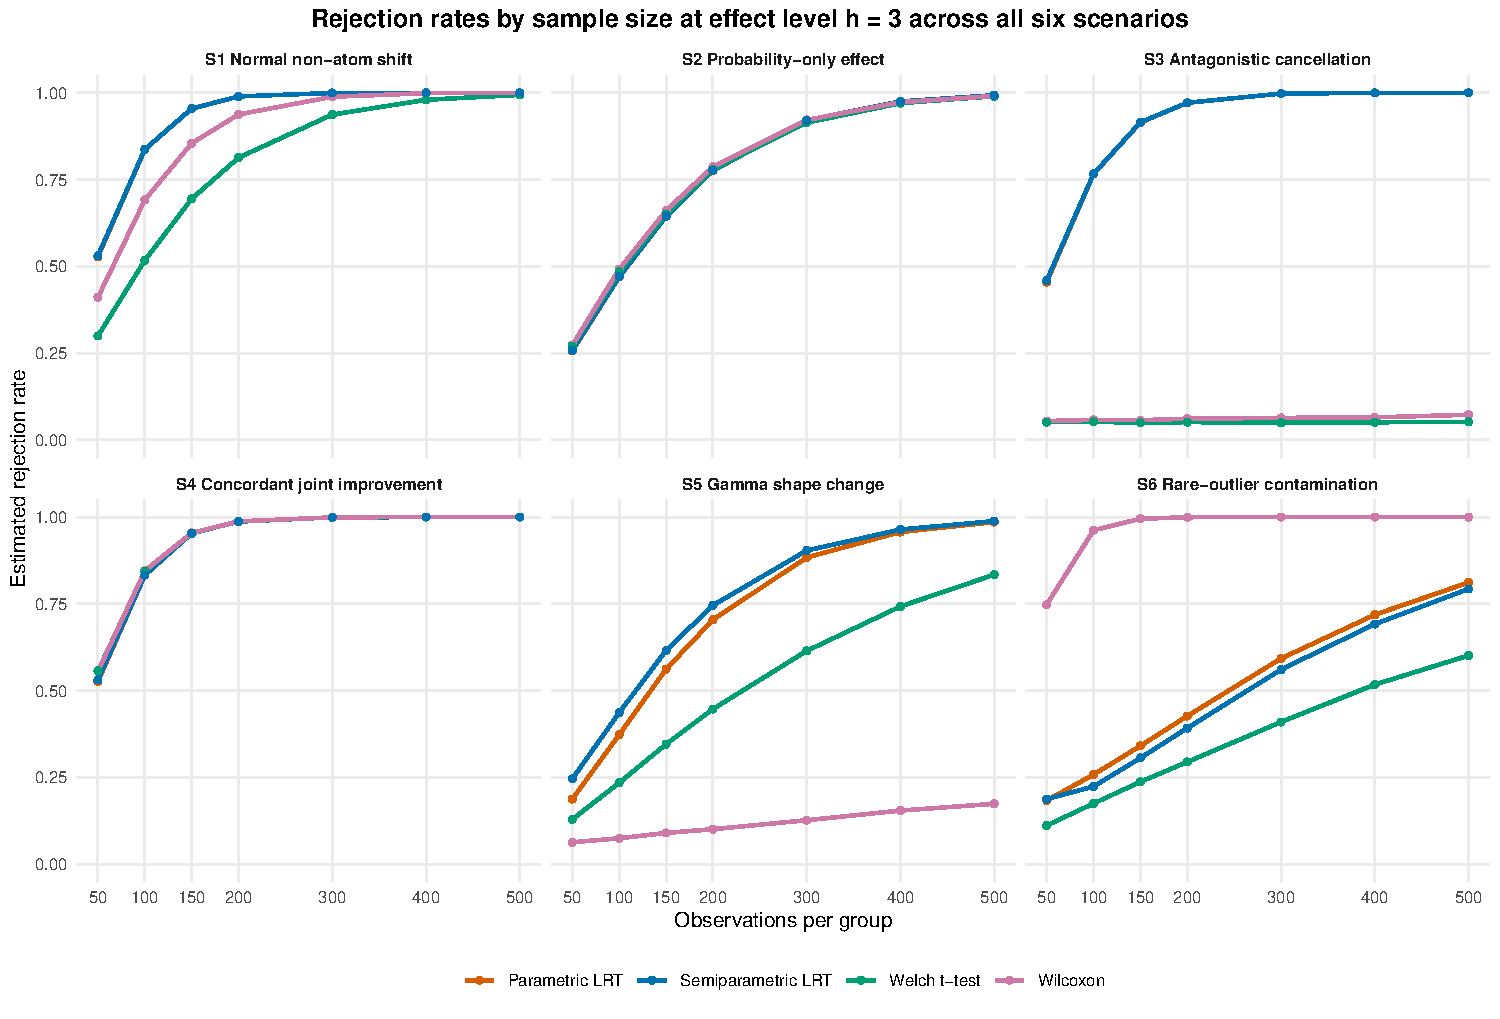
\includegraphics[width=0.84\textwidth]{power-curves.pdf}
\caption{Estimated power as a function of sample size at effect level $h=3$, the largest simulated departure from the null, for Scenarios~1 through~6.}
\label{fig:powerCurves}
\end{figure}

\begin{figure}[htbp]
\centering
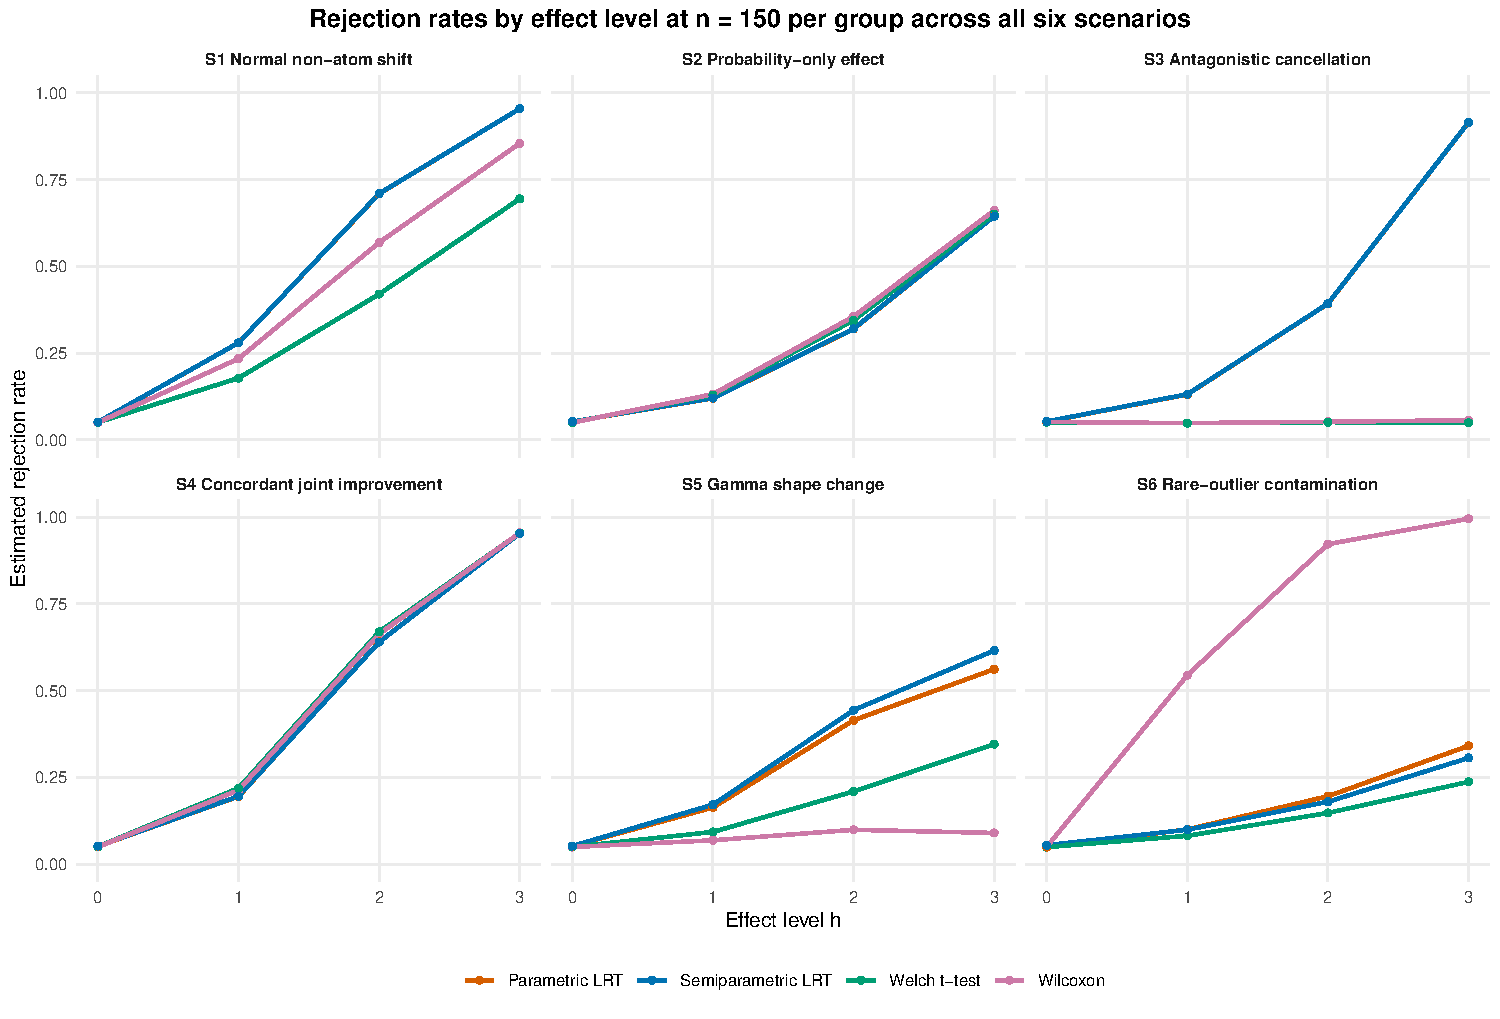
\includegraphics[width=0.84\textwidth]{power-effects.pdf}
\caption{Estimated power as a function of effect level at $n = 150$ observations per group for Scenarios~1 through~6.}
\label{fig:powerEffectCurves}
\end{figure}

The results support the main motivation for the proposed tests, but they also show that no single procedure is uniformly best. Scenario~1 is the reference case for the parametric assumptions: the survivor distribution is normal, the atom probability is unchanged, and treatment shifts the survivor mean. At $h=3$ and $n=150$, the likelihood-ratio tests rejected 95.4\% of replicates, compared with 85.4\% for Wilcoxon and 69.4\% for the $t$-test. In Scenario~2, where treatment acts only through the atom probability, all four procedures detected the effect similarly. The one-dimensional tests were slightly ahead at $n=150$ (66.1\% for Wilcoxon versus 64.4\% for either likelihood-ratio test), and by $n=500$ all four rejection rates were about 99\%.

Scenario~3 is the clearest verification of the two-component idea. In that antagonistic setting, the coded combined-outcome mean is fixed at every effect level even though the atom probability and survivor mean both change. At $h=3$ and $n=150$, the likelihood-ratio tests reached about 91.5\% power, whereas the Wilcoxon and $t$-tests remained near their null rejection rates. By $n=500$, both likelihood-ratio procedures rejected every replicate, while the one-dimensional tests still had little signal. Scenario~4 is the least discriminating non-null scenario for comparing methods: when both components improve concordantly, the effect is already visible on the coded combined-outcome scale, and all four methods have similar power.

The non-normal scenarios illustrate the role of the survivor distribution. In Scenario~5, the survivor distribution changes shape and mean. The semi-parametric likelihood-ratio test is consistently the most powerful procedure, the parametric likelihood-ratio test is close but lower, the $t$-test is intermediate, and Wilcoxon has poor power; at $h=3$ and $n=150$, the corresponding rejection rates were 61.5\%, 56.2\%, 34.6\%, and 9.0\%. Scenario~6 deliberately favors a rank test through rare outlier contamination. Wilcoxon therefore dominates, while the likelihood-ratio tests outperform the $t$-test but are not competitive with Wilcoxon; at $h=3$ and $n=150$, Wilcoxon rejected 99.5\% of replicates, compared with 34.1\% for the parametric likelihood-ratio test, 30.6\% for the semi-parametric likelihood-ratio test, and 23.7\% for the $t$-test.

The null-calibration results are mostly reassuring but not perfectly uniform. Across the full simulation run, all method failure rates were zero. Most null rejection rates were close to the nominal 5\% level for all four methods. The important exception was the semi-parametric likelihood-ratio test in the rare-outlier null setting: its rejection rate was 12.6\% at $n=50$ and 6.6\% at $n=100$, before settling near nominal from $n \ge 150$. Thus the main conclusions are strongest for moderate sample sizes, while very small contaminated samples require caution for the semi-parametric procedure. The long supplementary tables document the full scenario-by-sample-size patterns underlying Figure~\ref{fig:powerCurves}.

\section{Clinical application: IST-3 stroke trial}\label{sec:application}

We apply the proposed methods to \ApplicationDatasetDescription{} \citep{IST3Lancet2012,IST3DataShare}. Acute ischemic stroke is a natural setting for atom-plus-continuous endpoints: treatment may affect both mortality and functional health, and death before follow-up is not a missing quality-of-life value but a clinically meaningful terminal state. Among participants alive at 6 months with observed EQ-VAS, the EuroQol visual analogue score is a patient-centered measure on a 0 to 100 scale, with larger values indicating better self-rated health.

The IST-3 data were downloaded from Edinburgh DataShare. The fixed-width data file \texttt{ist3.dat} and accompanying SAS syntax identify allocated treatment, death by 6 months, and 6-month EQ-VAS. The syntax labels \texttt{itt\_treat} as allocated treatment, \texttt{dead6mo} as death before 6 months, and \texttt{euroqol6} as the 6-month EuroQol health state. We verified the treatment coding against the text treatment field: \texttt{itt\_treat = 0} corresponds to rt-PA and \texttt{itt\_treat = 1} corresponds to placebo/control. We therefore set $R=1$ for rt-PA and $R=0$ for placebo/control. The DataShare record is publicly downloadable after the end of the embargo, but reuse is conditional on the IST-3 Data Use Agreement; the data citation is \citet{IST3DataShare}, DOI \ApplicationISTThreeDoi{}.

For the application endpoint, first restrict to the analysis sample by excluding participants who were alive at 6 months but had missing EQ-VAS; deaths are retained through the atom. On this analysis sample, let
\[
  A=\mathbbm{1}\{\text{alive at 6 months with observed EQ-VAS}\}.
\]
For participants with $A=1$, let $Y^{\mathrm{EQVAS}}$ denote the observed 6-month EQ-VAS score. Define the abstract endpoint on the analysis sample by
\[
  \widetilde Y=
  \begin{cases}
    Y^{\mathrm{EQVAS}}, & A=1,\\
    \mathcal E, & \text{death by 6 months}.
  \end{cases}
\]
The coded endpoint used for numerical summaries is
\[
  \widetilde Y^{(-1)}=c_{-1}(\widetilde Y)=
  \begin{cases}
    Y^{\mathrm{EQVAS}}, & A=1,\\
    -1, & \text{death by 6 months}.
  \end{cases}
\]
Thus the abstract atom $\mathcal E$, representing death by 6 months, is coded as $e_0=-1$. Since the non-atom EQ-VAS scale is 0 to 100, this code lies outside the non-atom support, so the coded value $-1$ uniquely identifies the atom in this application. In this application, write $\Delta=\Delta^{(-1)}$. This left \ApplicationN{} participants for analysis, including \ApplicationControlN{} placebo/control participants and \ApplicationTreatmentN{} rt-PA participants. Table~\ref{tab:ist3-descriptives} reports the analysis sample, death counts, EQ-VAS summaries among those alive with observed scores, and the combined endpoint mean.

\input{build/tables/application-descriptives.tex}

Figure~\ref{fig:application} displays the atom and non-atom components together with the semiparametric joint confidence region. The death atom was similar in the two arms: \ApplicationControlDeaths{} placebo/control participants (\ApplicationControlDeathPct{}) and \ApplicationTreatmentDeaths{} rt-PA participants (\ApplicationTreatmentDeathPct{}) died before 6 months. Among participants alive with observed EQ-VAS, however, the mean was \ApplicationControlMean{} in the placebo/control arm and \ApplicationTreatmentMean{} in the rt-PA arm, giving $\hat\mu_\delta=\ApplicationMuDelta{}$ points. The fitted odds ratio for being alive with observed EQ-VAS rather than at the death atom was $\hat\alpha_\delta=\ApplicationAlphaDelta{}$, and the combined mean contrast $\Delta^{(-1)}$ under the death code $e_0=-1$ was $\hat\Delta=\ApplicationDelta{}$.

\begin{figure}[htbp]
\centering

\includegraphics[width=\textwidth]{application.pdf}
\caption{IST-3 endpoint decomposition and semiparametric likelihood-ratio region. The left panel shows, by treatment arm, deaths and participants alive with observed EQ-VAS. The middle panel shows the EQ-VAS distribution among participants alive with observed scores. The right panel shows the semiparametric likelihood-ratio surface for $(\mu_\delta,\log\alpha_\delta)$ with reference lines at no non-atom mean difference and no atom-probability difference.}
\label{fig:application}
\end{figure}

Table~\ref{tab:ist3-frequentist} compares standard one-dimensional analyses with the proposed joint tests. A Welch $t$-test applied directly to the coded endpoint $\widetilde Y^{(-1)}$ gave p-value \ApplicationTTestP{}, and the Wilcoxon rank-sum test gave p-value \ApplicationWilcoxP{}. The $t$-test on $\widetilde Y^{(-1)}$ depends on the numerical code $e_0=-1$ for death; moving the death code would change the mean contrast and its standard error. The Wilcoxon test is less tied to that exact value, but it treats all deaths as tied observations at the worst rank and still collapses the endpoint to one dimension. An analysis restricted to participants alive with observed EQ-VAS is more sensitive to the EQ-VAS difference, but it conditions on a post-randomization alive-at-follow-up event and therefore answers a different observed-data question.

\input{build/tables/application-frequentist.tex}

The likelihood-ratio procedures test the joint null of no treatment effect on the death atom probability and no treatment effect on non-atom EQ-VAS. The parametric LRT statistic was \ApplicationLRTStatistic{} with p-value \ApplicationLRTP{}, and the semiparametric LRT statistic was \ApplicationSPLRTStatistic{} with p-value \ApplicationSPLRTP{}. In this data set the two procedures agree closely, suggesting that the signal is mainly a location shift in the EQ-VAS component rather than a feature driven by the parametric distributional assumption. Clinically, $\mu_\delta$ is the rt-PA minus control mean EQ-VAS difference among participants alive with observed scores; $\alpha_\delta$ is the rt-PA/control odds ratio for being alive with observed EQ-VAS rather than at the death atom; and $\Delta$ is the rt-PA minus control mean of the combined endpoint under the death code $e_0=-1$. The joint rejection should therefore be interpreted as evidence that the observed two-component endpoint distribution differs between randomized arms, not as a principal-stratum causal effect.

For the combined mean contrast $\Delta=\Delta^{(-1)}$, the direct Welch interval for $\widetilde Y^{(-1)}$ was $[-0.46, 4.63]$, and the semiparametric profile-likelihood interval was almost identical at $[-0.46, 4.62]$. By contrast, projecting the joint confidence region for the atom and non-atom components onto the $\Delta$ scale gave the wider interval $[-1.09, 5.25]$, reflecting the additional uncertainty retained by the two-component likelihood-ratio region.

We also fit a Bayesian two-part model using the bounded-score logit-Normal likelihood defined in Section~\ref{sec:bayesian-two-group}. The Bernoulli atom probabilities used independent $\mathrm{Beta}(1,1)$ priors. The non-atom EQ-VAS distribution used $H=2$ mixture components, score range 0 to 100, unit score spacing, ordered component locations on the logit scale, and shared heap weights over 1-, 5-, and 10-point reporting grids. The reporting-grid component was empirically relevant: among participants alive with observed EQ-VAS, 85.3\% of placebo/control scores and 83.8\% of rt-PA scores were multiples of 5, including 64.3\% and 62.7\%, respectively, that were multiples of 10. The stick-breaking concentration parameters used $\mathrm{Gamma}(4,4)$ priors, the logit-scale component locations used $\mathrm{Normal}(0,2)$ priors, the component scales used $\mathrm{Lognormal}(\log 1.2, 0.5)$ priors, and the heap weights used a $\mathrm{Dirichlet}(2,2,2)$ prior. Posterior computation used four chains with 1{,}000 warmup and 2{,}000 post-warmup iterations per chain, with target acceptance probability 0.995. Because this analysis uses a practical finite mixture, we report sampler and mixture-weight diagnostics alongside the posterior summaries.

\input{build/tables/application-bayes-summary.tex}

The posterior summaries in Table~\ref{tab:ist3-bayes} separate the atom/alive component from the non-atom EQ-VAS component. The benefit-oriented combined endpoint uses the same coding as the frequentist analysis, so $\Pr(\Delta>0\mid\mathrm{data})$ is the posterior probability that rt-PA improves the combined endpoint. The posterior probabilities $\Pr(\mu_\delta>0\mid\mathrm{data})$ and $\Pr(\alpha_\delta>1\mid\mathrm{data})$ separately summarize benefit on EQ-VAS among participants alive with observed scores and on avoiding the atom. Figure~\ref{fig:application-posterior} shows the posterior densities for these component and combined contrasts.

\begin{figure}[htbp]
\centering

\includegraphics[width=0.92\textwidth]{application-posterior.pdf}
\caption{Posterior distributions for the IST-3 treatment contrasts. Vertical dashed lines mark no non-atom mean difference, no difference in the odds of being alive with observed EQ-VAS, and no combined endpoint mean difference.}
\label{fig:application-posterior}
\end{figure}

Finally, we assessed whether the Bayesian model reproduced both parts of the endpoint. Using 200 posterior predictive draws, the maximum armwise absolute atom-rate deviation gave posterior predictive $p=0.545$, and the maximum armwise discrete CDF discrepancy for reported EQ-VAS scores gave posterior predictive $p=0.325$. These checks do not indicate a strong mismatch for either the death atom or the bounded, heaped non-atom EQ-VAS distribution; Figure~\ref{fig:application-ppc} gives a plot of the posterior predictive checks. The reported-score check therefore compares replicated and observed non-atom distributions as a model check, not as evidence for treatment efficacy.

\begin{figure}[htbp]
\centering

\includegraphics[width=\textwidth]{application-ppc.pdf}
\caption{Posterior predictive checks for the IST-3 Bayesian model, separately for the death atom and the non-atom EQ-VAS component. Gray bars show observed proportions and black points with vertical ranges show posterior predictive means and intervals; the left panel uses the death indicator by arm, whereas the right panel uses reported-score probability masses among participants alive with observed EQ-VAS. The p-values are model-checking p-values for the component-specific nulls that the fitted model reproduces the arm-specific death probabilities and the arm-specific non-atom reported-score distribution.}
\label{fig:application-ppc}
\end{figure}

\section{Discussion}\label{sec:discussion}

We have proposed parametric and semi-parametric likelihood-ratio tests for continuous outcomes with a clinically meaningful atom. The key step is to retain the atomized outcome used in practice while testing the joint null of no treatment effect on the atom probability and no treatment effect on the non-atom component. This yields one prespecified p-value together with interpretable component-wise effect estimates and confidence regions.

The simulations show why that distinction matters. The clearest gain appears when the atom and non-atom component move in opposite directions, because that is the setting in which a one-dimensional composite can cancel real component-level signal. When only the atom probability changes or when both components move concordantly, one-dimensional tests can be similarly powerful. The IST-3 application serves the same purpose in a clinically recognizable setting: the joint tests detect two-component structure that is only weakly visible to standard analyses of the raw combined outcome.

This observed-data focus should also guide interpretation. The parameter pair $(\mu_\delta,\beta_\delta)$ is not a survivor-average causal effect or a principal-stratum estimand; it describes the two components of the observed outcome distribution under randomization. The procedures are asymptotic, require positive numbers of observed outcomes in both groups, and the parametric version is only as credible as the model specified for $Y \mid A = 1$. The semi-parametric version relaxes that distributional assumption, but it still relies on regularity of the Bernoulli model and on feasible empirical-likelihood constraints.

For trials that require a single prespecified primary analysis, the framework offers one joint p-value together with clinically interpretable follow-up summaries for the binary and continuous components. That makes it attractive when investigators want to preserve the meaning of a worst-rank endpoint or atom-at-zero coding without collapsing the scientific question to a single distribution on the combined scale.

Software implementing both procedures, including the code used to generate the manuscript analyses, is available on GitHub \citep{TruncCompGitHub}.

\clearpage
\appendix
\section{Supplementary simulation results}\label{app:supplementary-simulation-results}

This appendix records additional details needed to reproduce the simulation study in Section~\ref{sec:simulation-study} and gives the full numerical results underlying the summary figures in the main text.

For each scenario--effect--sample-size cell, the random-number seed was set to $20260416$ plus the cell index minus one, with the cell index increasing first over scenarios, then over effect levels, and then over sample sizes. Each replicate was analyzed using four procedures: the Wilcoxon rank-sum test, Welch's two-sample $t$-test, the parametric likelihood-ratio test, and the semi-parametric likelihood-ratio test. A replicate was counted as a method failure if the corresponding analysis did not return a finite p-value; otherwise rejection was recorded according to whether the p-value was below $0.05$. The aggregated simulation output also retained method-specific failure rates and runtimes.

Figure~\ref{fig:type1Curves} gives the full null-calibration display for the $h=0$ cells. The tables that follow give the complete scenario-specific rejection rates across all simulated effect levels and sample sizes, together with the expected coded combined-outcome contrast used in the simulation summaries.

\begin{figure}[htbp]
\centering
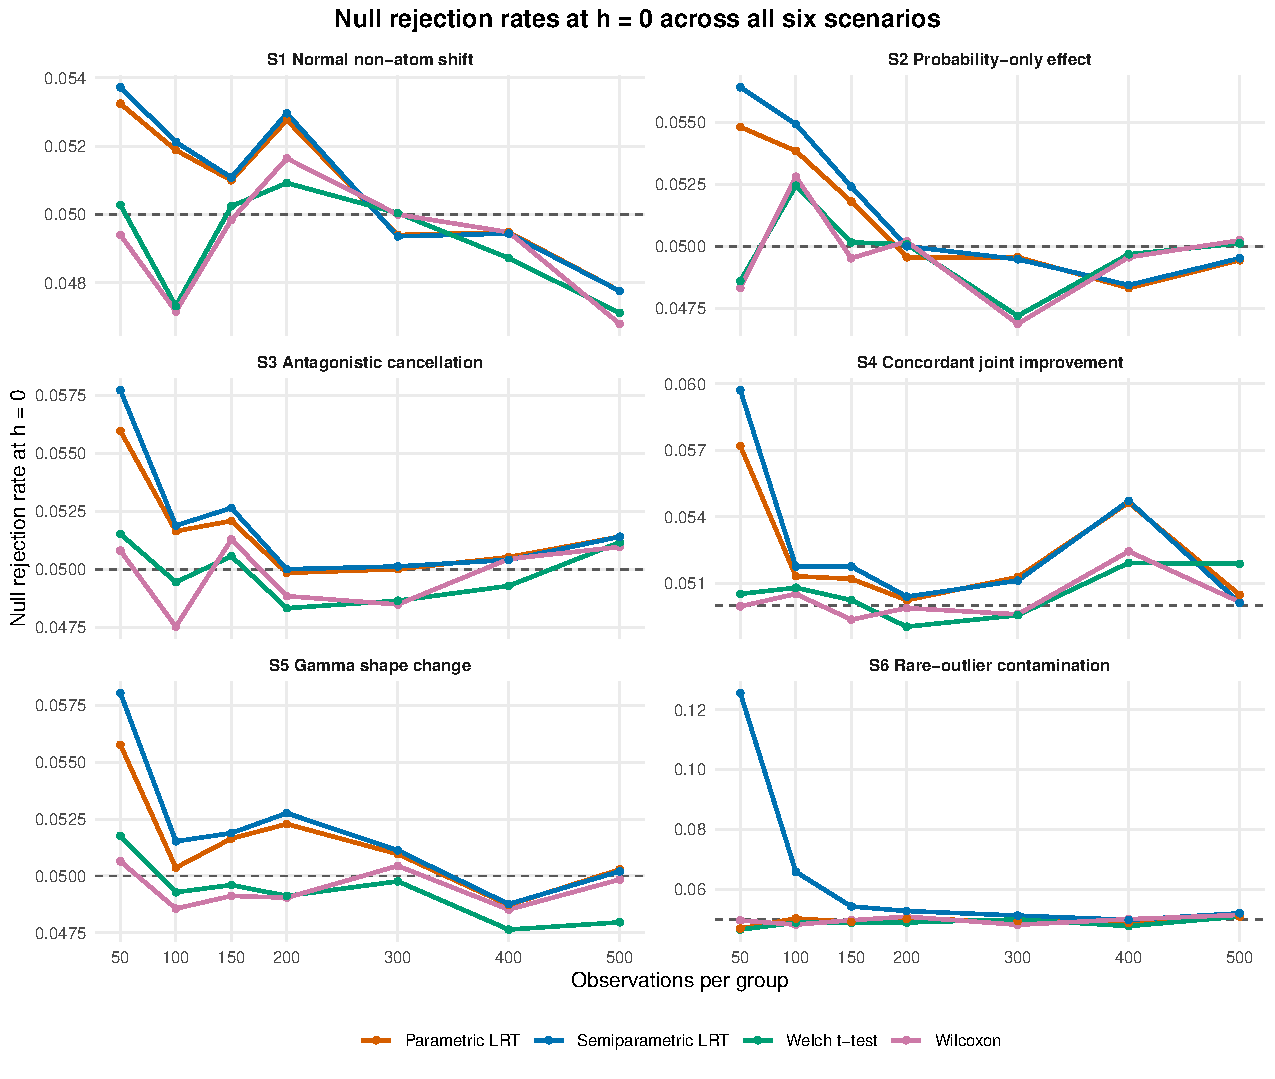
\includegraphics[width=0.84\textwidth]{type1-curves.pdf}
\caption{Null rejection rates at effect level $h = 0$ across all six simulation scenarios. The dashed line marks 0.05.}
\label{fig:type1Curves}
\end{figure}

\begingroup\fontsize{7}{9}\selectfont

\begin{longtable}[t]{rrlrrrrr}
\caption{Scenario S1 (Normal non-atom shift, low atom probability): estimated rejection percentages by sample size and effect level}\\
\toprule
$n_{\mathrm{arm}}$ & $h$ & Effect & Expected $\Delta^{(0)}$ & Wilcoxon (\%) & Welch $t$-test (\%) & LRT (\%) & SPLRT (\%)\\
\midrule
\endfirsthead
\caption[]{Scenario S1 (Normal non-atom shift, low atom probability): estimated rejection percentages by sample size and effect level \textit{(continued)}}\\
\toprule
$n_{\mathrm{arm}}$ & $h$ & Effect & Expected $\Delta^{(0)}$ & Wilcoxon (\%) & Welch $t$-test (\%) & LRT (\%) & SPLRT (\%)\\
\midrule
\endhead

\endfoot
\bottomrule
\endlastfoot
50 & 0 & \makecell[l]{$\delta_h = 0.00$} & 0.000 & 4.94 & 5.03 & 5.32 & 5.37\\
100 & 0 & \makecell[l]{$\delta_h = 0.00$} & 0.000 & 4.72 & 4.73 & 5.19 & 5.21\\
150 & 0 & \makecell[l]{$\delta_h = 0.00$} & 0.000 & 4.98 & 5.02 & 5.10 & 5.11\\
200 & 0 & \makecell[l]{$\delta_h = 0.00$} & 0.000 & 5.16 & 5.09 & 5.28 & 5.30\\
300 & 0 & \makecell[l]{$\delta_h = 0.00$} & 0.000 & 5.00 & 5.00 & 4.94 & 4.94\\
400 & 0 & \makecell[l]{$\delta_h = 0.00$} & 0.000 & 4.95 & 4.87 & 4.95 & 4.94\\
500 & 0 & \makecell[l]{$\delta_h = 0.00$} & 0.000 & 4.68 & 4.71 & 4.78 & 4.78\\
50 & 1 & \makecell[l]{$\delta_h = 0.20$} & 0.170 & 10.65 & 9.25 & 12.44 & 12.56\\
100 & 1 & \makecell[l]{$\delta_h = 0.20$} & 0.170 & 16.89 & 13.26 & 20.16 & 20.17\\
150 & 1 & \makecell[l]{$\delta_h = 0.20$} & 0.170 & 23.37 & 17.78 & 27.97 & 27.97\\
200 & 1 & \makecell[l]{$\delta_h = 0.20$} & 0.170 & 29.32 & 21.86 & 35.98 & 36.01\\
300 & 1 & \makecell[l]{$\delta_h = 0.20$} & 0.170 & 40.84 & 30.20 & 50.76 & 50.78\\
400 & 1 & \makecell[l]{$\delta_h = 0.20$} & 0.170 & 52.36 & 39.04 & 64.54 & 64.60\\
500 & 1 & \makecell[l]{$\delta_h = 0.20$} & 0.170 & 60.72 & 45.90 & 74.45 & 74.40\\
50 & 2 & \makecell[l]{$\delta_h = 0.35$} & 0.298 & 22.98 & 17.55 & 28.78 & 29.02\\
100 & 2 & \makecell[l]{$\delta_h = 0.35$} & 0.298 & 41.03 & 30.20 & 51.88 & 52.00\\
150 & 2 & \makecell[l]{$\delta_h = 0.35$} & 0.298 & 56.84 & 41.98 & 70.91 & 70.96\\
200 & 2 & \makecell[l]{$\delta_h = 0.35$} & 0.298 & 69.77 & 53.36 & 83.26 & 83.22\\
300 & 2 & \makecell[l]{$\delta_h = 0.35$} & 0.298 & 85.27 & 69.76 & 95.02 & 95.03\\
400 & 2 & \makecell[l]{$\delta_h = 0.35$} & 0.298 & 93.56 & 81.58 & 98.80 & 98.80\\
500 & 2 & \makecell[l]{$\delta_h = 0.35$} & 0.298 & 97.37 & 89.66 & 99.76 & 99.76\\
50 & 3 & \makecell[l]{$\delta_h = 0.50$} & 0.425 & 41.04 & 29.95 & 52.75 & 53.05\\
100 & 3 & \makecell[l]{$\delta_h = 0.50$} & 0.425 & 69.14 & 51.71 & 83.67 & 83.70\\
150 & 3 & \makecell[l]{$\delta_h = 0.50$} & 0.425 & 85.45 & 69.44 & 95.45 & 95.44\\
200 & 3 & \makecell[l]{$\delta_h = 0.50$} & 0.425 & 93.76 & 81.30 & 98.95 & 98.95\\
300 & 3 & \makecell[l]{$\delta_h = 0.50$} & 0.425 & 98.86 & 93.72 & 99.94 & 99.94\\
400 & 3 & \makecell[l]{$\delta_h = 0.50$} & 0.425 & 99.88 & 97.97 & 100.00 & 100.00\\
500 & 3 & \makecell[l]{$\delta_h = 0.50$} & 0.425 & 99.98 & 99.40 & 100.00 & 100.00\\*
\end{longtable}
\endgroup{}

\begingroup\fontsize{7}{9}\selectfont

\begin{longtable}[t]{rrlrrrrr}
\caption{Scenario S2 (effect only on probability outside atom): estimated rejection percentages by sample size and effect level}\\
\toprule
$n_{\mathrm{arm}}$ & $h$ & Effect & Expected $\Delta^{(0)}$ & Wilcoxon (\%) & Welch $t$-test (\%) & LRT (\%) & SPLRT (\%)\\
\midrule
\endfirsthead
\caption[]{Scenario S2 (effect only on probability outside atom): estimated rejection percentages by sample size and effect level \textit{(continued)}}\\
\toprule
$n_{\mathrm{arm}}$ & $h$ & Effect & Expected $\Delta^{(0)}$ & Wilcoxon (\%) & Welch $t$-test (\%) & LRT (\%) & SPLRT (\%)\\
\midrule
\endhead

\endfoot
\bottomrule
\endlastfoot
50 & 0 & \makecell[l]{$\pi_{1,h} = 0.45$} & 0.00 & 4.83 & 4.86 & 5.48 & 5.64\\
100 & 0 & \makecell[l]{$\pi_{1,h} = 0.45$} & 0.00 & 5.28 & 5.24 & 5.38 & 5.49\\
150 & 0 & \makecell[l]{$\pi_{1,h} = 0.45$} & 0.00 & 4.95 & 5.02 & 5.18 & 5.24\\
200 & 0 & \makecell[l]{$\pi_{1,h} = 0.45$} & 0.00 & 5.02 & 5.01 & 4.96 & 5.00\\
300 & 0 & \makecell[l]{$\pi_{1,h} = 0.45$} & 0.00 & 4.69 & 4.72 & 4.96 & 4.95\\
400 & 0 & \makecell[l]{$\pi_{1,h} = 0.45$} & 0.00 & 4.96 & 4.97 & 4.83 & 4.84\\
500 & 0 & \makecell[l]{$\pi_{1,h} = 0.45$} & 0.00 & 5.02 & 5.01 & 4.94 & 4.95\\
50 & 1 & \makecell[l]{$\pi_{1,h} = 0.50$} & 0.15 & 7.70 & 7.74 & 7.74 & 7.91\\
100 & 1 & \makecell[l]{$\pi_{1,h} = 0.50$} & 0.15 & 9.90 & 9.76 & 9.04 & 9.04\\
150 & 1 & \makecell[l]{$\pi_{1,h} = 0.50$} & 0.15 & 13.13 & 12.89 & 11.96 & 12.01\\
200 & 1 & \makecell[l]{$\pi_{1,h} = 0.50$} & 0.15 & 15.28 & 14.79 & 13.08 & 13.09\\
300 & 1 & \makecell[l]{$\pi_{1,h} = 0.50$} & 0.15 & 20.23 & 19.51 & 17.86 & 17.88\\
400 & 1 & \makecell[l]{$\pi_{1,h} = 0.50$} & 0.15 & 26.26 & 25.10 & 22.88 & 22.90\\
500 & 1 & \makecell[l]{$\pi_{1,h} = 0.50$} & 0.15 & 31.61 & 30.40 & 27.64 & 27.64\\
50 & 2 & \makecell[l]{$\pi_{1,h} = 0.55$} & 0.30 & 14.73 & 14.51 & 13.93 & 14.15\\
100 & 2 & \makecell[l]{$\pi_{1,h} = 0.55$} & 0.30 & 25.27 & 24.69 & 23.11 & 23.11\\
150 & 2 & \makecell[l]{$\pi_{1,h} = 0.55$} & 0.30 & 35.54 & 34.42 & 31.94 & 31.98\\
200 & 2 & \makecell[l]{$\pi_{1,h} = 0.55$} & 0.30 & 45.40 & 43.97 & 41.52 & 41.54\\
300 & 2 & \makecell[l]{$\pi_{1,h} = 0.55$} & 0.30 & 61.90 & 60.21 & 58.91 & 58.90\\
400 & 2 & \makecell[l]{$\pi_{1,h} = 0.55$} & 0.30 & 74.22 & 72.58 & 71.88 & 71.86\\
500 & 2 & \makecell[l]{$\pi_{1,h} = 0.55$} & 0.30 & 83.02 & 81.57 & 81.38 & 81.39\\
50 & 3 & \makecell[l]{$\pi_{1,h} = 0.60$} & 0.45 & 27.30 & 27.02 & 25.59 & 25.84\\
100 & 3 & \makecell[l]{$\pi_{1,h} = 0.60$} & 0.45 & 49.18 & 48.44 & 46.92 & 47.00\\
150 & 3 & \makecell[l]{$\pi_{1,h} = 0.60$} & 0.45 & 66.08 & 64.98 & 64.40 & 64.39\\
200 & 3 & \makecell[l]{$\pi_{1,h} = 0.60$} & 0.45 & 78.67 & 77.90 & 77.57 & 77.59\\
300 & 3 & \makecell[l]{$\pi_{1,h} = 0.60$} & 0.45 & 92.17 & 91.39 & 92.10 & 92.10\\
400 & 3 & \makecell[l]{$\pi_{1,h} = 0.60$} & 0.45 & 97.29 & 97.01 & 97.50 & 97.50\\
500 & 3 & \makecell[l]{$\pi_{1,h} = 0.60$} & 0.45 & 99.09 & 99.00 & 99.30 & 99.30\\*
\end{longtable}
\endgroup{}

\begingroup\fontsize{7}{9}\selectfont

\begin{longtable}[t]{rrlrrrrr}
\caption{Scenario S3 (antagonistic cancellation): estimated rejection percentages by sample size and effect level}\\
\toprule
$n_{\mathrm{arm}}$ & $h$ & Effect & Expected $\Delta^{(0)}$ & Wilcoxon (\%) & Welch $t$-test (\%) & LRT (\%) & SPLRT (\%)\\
\midrule
\endfirsthead
\caption[]{Scenario S3 (antagonistic cancellation): estimated rejection percentages by sample size and effect level \textit{(continued)}}\\
\toprule
$n_{\mathrm{arm}}$ & $h$ & Effect & Expected $\Delta^{(0)}$ & Wilcoxon (\%) & Welch $t$-test (\%) & LRT (\%) & SPLRT (\%)\\
\midrule
\endhead

\endfoot
\bottomrule
\endlastfoot
50 & 0 & \makecell[l]{$\pi_{1,h} = 0.500$, $1.5 / \pi_{1,h} = 3.000$} & 0 & 5.08 & 5.15 & 5.60 & 5.77\\
100 & 0 & \makecell[l]{$\pi_{1,h} = 0.500$, $1.5 / \pi_{1,h} = 3.000$} & 0 & 4.75 & 4.94 & 5.16 & 5.19\\
150 & 0 & \makecell[l]{$\pi_{1,h} = 0.500$, $1.5 / \pi_{1,h} = 3.000$} & 0 & 5.13 & 5.06 & 5.21 & 5.26\\
200 & 0 & \makecell[l]{$\pi_{1,h} = 0.500$, $1.5 / \pi_{1,h} = 3.000$} & 0 & 4.88 & 4.83 & 4.98 & 5.00\\
300 & 0 & \makecell[l]{$\pi_{1,h} = 0.500$, $1.5 / \pi_{1,h} = 3.000$} & 0 & 4.85 & 4.86 & 5.00 & 5.01\\
400 & 0 & \makecell[l]{$\pi_{1,h} = 0.500$, $1.5 / \pi_{1,h} = 3.000$} & 0 & 5.04 & 4.93 & 5.05 & 5.04\\
500 & 0 & \makecell[l]{$\pi_{1,h} = 0.500$, $1.5 / \pi_{1,h} = 3.000$} & 0 & 5.10 & 5.12 & 5.14 & 5.14\\
50 & 1 & \makecell[l]{$\pi_{1,h} = 0.525$, $1.5 / \pi_{1,h} = 2.857$} & 0 & 5.10 & 5.16 & 8.12 & 8.39\\
100 & 1 & \makecell[l]{$\pi_{1,h} = 0.525$, $1.5 / \pi_{1,h} = 2.857$} & 0 & 4.92 & 4.94 & 10.43 & 10.46\\
150 & 1 & \makecell[l]{$\pi_{1,h} = 0.525$, $1.5 / \pi_{1,h} = 2.857$} & 0 & 4.81 & 4.80 & 13.06 & 13.12\\
200 & 1 & \makecell[l]{$\pi_{1,h} = 0.525$, $1.5 / \pi_{1,h} = 2.857$} & 0 & 5.01 & 4.99 & 16.37 & 16.44\\
300 & 1 & \makecell[l]{$\pi_{1,h} = 0.525$, $1.5 / \pi_{1,h} = 2.857$} & 0 & 4.90 & 4.86 & 21.46 & 21.48\\
400 & 1 & \makecell[l]{$\pi_{1,h} = 0.525$, $1.5 / \pi_{1,h} = 2.857$} & 0 & 5.15 & 5.03 & 28.53 & 28.52\\
500 & 1 & \makecell[l]{$\pi_{1,h} = 0.525$, $1.5 / \pi_{1,h} = 2.857$} & 0 & 5.08 & 4.99 & 34.50 & 34.49\\
50 & 2 & \makecell[l]{$\pi_{1,h} = 0.550$, $1.5 / \pi_{1,h} = 2.727$} & 0 & 4.74 & 4.92 & 15.72 & 16.10\\
100 & 2 & \makecell[l]{$\pi_{1,h} = 0.550$, $1.5 / \pi_{1,h} = 2.727$} & 0 & 5.33 & 5.22 & 27.74 & 27.78\\
150 & 2 & \makecell[l]{$\pi_{1,h} = 0.550$, $1.5 / \pi_{1,h} = 2.727$} & 0 & 5.19 & 5.06 & 39.20 & 39.23\\
200 & 2 & \makecell[l]{$\pi_{1,h} = 0.550$, $1.5 / \pi_{1,h} = 2.727$} & 0 & 5.12 & 4.99 & 49.88 & 49.83\\
300 & 2 & \makecell[l]{$\pi_{1,h} = 0.550$, $1.5 / \pi_{1,h} = 2.727$} & 0 & 5.51 & 5.10 & 68.10 & 68.15\\
400 & 2 & \makecell[l]{$\pi_{1,h} = 0.550$, $1.5 / \pi_{1,h} = 2.727$} & 0 & 5.60 & 5.09 & 80.76 & 80.78\\
500 & 2 & \makecell[l]{$\pi_{1,h} = 0.550$, $1.5 / \pi_{1,h} = 2.727$} & 0 & 5.56 & 5.10 & 89.15 & 89.10\\
50 & 3 & \makecell[l]{$\pi_{1,h} = 0.600$, $1.5 / \pi_{1,h} = 2.500$} & 0 & 5.41 & 5.06 & 45.44 & 45.90\\
100 & 3 & \makecell[l]{$\pi_{1,h} = 0.600$, $1.5 / \pi_{1,h} = 2.500$} & 0 & 5.71 & 5.20 & 76.60 & 76.64\\
150 & 3 & \makecell[l]{$\pi_{1,h} = 0.600$, $1.5 / \pi_{1,h} = 2.500$} & 0 & 5.65 & 4.88 & 91.47 & 91.49\\
200 & 3 & \makecell[l]{$\pi_{1,h} = 0.600$, $1.5 / \pi_{1,h} = 2.500$} & 0 & 6.06 & 5.08 & 97.12 & 97.12\\
300 & 3 & \makecell[l]{$\pi_{1,h} = 0.600$, $1.5 / \pi_{1,h} = 2.500$} & 0 & 6.32 & 4.93 & 99.78 & 99.78\\
400 & 3 & \makecell[l]{$\pi_{1,h} = 0.600$, $1.5 / \pi_{1,h} = 2.500$} & 0 & 6.46 & 5.04 & 99.97 & 99.97\\
500 & 3 & \makecell[l]{$\pi_{1,h} = 0.600$, $1.5 / \pi_{1,h} = 2.500$} & 0 & 7.22 & 5.14 & 100.00 & 100.00\\*
\end{longtable}
\endgroup{}

\begingroup\fontsize{7}{9}\selectfont

\begin{longtable}[t]{rrlrrrrr}
\caption{Scenario S4 (concordant joint improvement): estimated rejection percentages by sample size and effect level}\\
\toprule
$n_{\mathrm{arm}}$ & $h$ & Effect & Expected $\Delta^{(0)}$ & Wilcoxon (\%) & Welch $t$-test (\%) & LRT (\%) & SPLRT (\%)\\
\midrule
\endfirsthead
\caption[]{Scenario S4 (concordant joint improvement): estimated rejection percentages by sample size and effect level \textit{(continued)}}\\
\toprule
$n_{\mathrm{arm}}$ & $h$ & Effect & Expected $\Delta^{(0)}$ & Wilcoxon (\%) & Welch $t$-test (\%) & LRT (\%) & SPLRT (\%)\\
\midrule
\endhead

\endfoot
\bottomrule
\endlastfoot
50 & 0 & \makecell[l]{$\pi_{1,h} = 0.50$, $3 + 0.15h = 3.00$} & 0.000 & 5.00 & 5.05 & 5.72 & 5.97\\
100 & 0 & \makecell[l]{$\pi_{1,h} = 0.50$, $3 + 0.15h = 3.00$} & 0.000 & 5.05 & 5.08 & 5.13 & 5.18\\
150 & 0 & \makecell[l]{$\pi_{1,h} = 0.50$, $3 + 0.15h = 3.00$} & 0.000 & 4.94 & 5.02 & 5.12 & 5.18\\
200 & 0 & \makecell[l]{$\pi_{1,h} = 0.50$, $3 + 0.15h = 3.00$} & 0.000 & 4.99 & 4.90 & 5.02 & 5.04\\
300 & 0 & \makecell[l]{$\pi_{1,h} = 0.50$, $3 + 0.15h = 3.00$} & 0.000 & 4.96 & 4.96 & 5.13 & 5.11\\
400 & 0 & \makecell[l]{$\pi_{1,h} = 0.50$, $3 + 0.15h = 3.00$} & 0.000 & 5.24 & 5.19 & 5.46 & 5.47\\
500 & 0 & \makecell[l]{$\pi_{1,h} = 0.50$, $3 + 0.15h = 3.00$} & 0.000 & 5.02 & 5.19 & 5.05 & 5.01\\
50 & 1 & \makecell[l]{$\pi_{1,h} = 0.55$, $3 + 0.15h = 3.15$} & 0.233 & 10.04 & 10.37 & 9.84 & 10.07\\
100 & 1 & \makecell[l]{$\pi_{1,h} = 0.55$, $3 + 0.15h = 3.15$} & 0.233 & 15.71 & 16.25 & 14.39 & 14.47\\
150 & 1 & \makecell[l]{$\pi_{1,h} = 0.55$, $3 + 0.15h = 3.15$} & 0.233 & 21.30 & 21.88 & 19.48 & 19.54\\
200 & 1 & \makecell[l]{$\pi_{1,h} = 0.55$, $3 + 0.15h = 3.15$} & 0.233 & 26.52 & 27.40 & 24.43 & 24.40\\
300 & 1 & \makecell[l]{$\pi_{1,h} = 0.55$, $3 + 0.15h = 3.15$} & 0.233 & 37.70 & 38.72 & 34.90 & 34.93\\
400 & 1 & \makecell[l]{$\pi_{1,h} = 0.55$, $3 + 0.15h = 3.15$} & 0.233 & 48.14 & 49.66 & 45.59 & 45.53\\
500 & 1 & \makecell[l]{$\pi_{1,h} = 0.55$, $3 + 0.15h = 3.15$} & 0.233 & 56.48 & 57.87 & 54.23 & 54.19\\
50 & 2 & \makecell[l]{$\pi_{1,h} = 0.60$, $3 + 0.15h = 3.30$} & 0.480 & 27.45 & 28.01 & 25.71 & 26.04\\
100 & 2 & \makecell[l]{$\pi_{1,h} = 0.60$, $3 + 0.15h = 3.30$} & 0.480 & 48.84 & 49.53 & 46.02 & 46.10\\
150 & 2 & \makecell[l]{$\pi_{1,h} = 0.60$, $3 + 0.15h = 3.30$} & 0.480 & 66.29 & 66.94 & 64.03 & 63.99\\
200 & 2 & \makecell[l]{$\pi_{1,h} = 0.60$, $3 + 0.15h = 3.30$} & 0.480 & 78.16 & 78.66 & 76.47 & 76.44\\
300 & 2 & \makecell[l]{$\pi_{1,h} = 0.60$, $3 + 0.15h = 3.30$} & 0.480 & 91.95 & 92.20 & 91.80 & 91.84\\
400 & 2 & \makecell[l]{$\pi_{1,h} = 0.60$, $3 + 0.15h = 3.30$} & 0.480 & 97.39 & 97.56 & 97.56 & 97.56\\
500 & 2 & \makecell[l]{$\pi_{1,h} = 0.60$, $3 + 0.15h = 3.30$} & 0.480 & 99.20 & 99.27 & 99.33 & 99.33\\
50 & 3 & \makecell[l]{$\pi_{1,h} = 0.65$, $3 + 0.15h = 3.45$} & 0.743 & 55.57 & 55.71 & 52.62 & 53.11\\
100 & 3 & \makecell[l]{$\pi_{1,h} = 0.65$, $3 + 0.15h = 3.45$} & 0.743 & 84.54 & 84.45 & 83.25 & 83.26\\
150 & 3 & \makecell[l]{$\pi_{1,h} = 0.65$, $3 + 0.15h = 3.45$} & 0.743 & 95.45 & 95.40 & 95.32 & 95.32\\
200 & 3 & \makecell[l]{$\pi_{1,h} = 0.65$, $3 + 0.15h = 3.45$} & 0.743 & 98.77 & 98.69 & 98.76 & 98.74\\
300 & 3 & \makecell[l]{$\pi_{1,h} = 0.65$, $3 + 0.15h = 3.45$} & 0.743 & 99.92 & 99.92 & 99.91 & 99.91\\
400 & 3 & \makecell[l]{$\pi_{1,h} = 0.65$, $3 + 0.15h = 3.45$} & 0.743 & 100.00 & 100.00 & 100.00 & 100.00\\
500 & 3 & \makecell[l]{$\pi_{1,h} = 0.65$, $3 + 0.15h = 3.45$} & 0.743 & 100.00 & 100.00 & 100.00 & 100.00\\*
\end{longtable}
\endgroup{}

\begingroup\fontsize{7}{9}\selectfont

\begin{longtable}[t]{rrlrrrrr}
\caption{Scenario S5 (Gamma shape change with non-atom mean shift): estimated rejection percentages by sample size and effect level}\\
\toprule
$n_{\mathrm{arm}}$ & $h$ & Effect & Expected $\Delta^{(0)}$ & Wilcoxon (\%) & Welch $t$-test (\%) & LRT (\%) & SPLRT (\%)\\
\midrule
\endfirsthead
\caption[]{Scenario S5 (Gamma shape change with non-atom mean shift): estimated rejection percentages by sample size and effect level \textit{(continued)}}\\
\toprule
$n_{\mathrm{arm}}$ & $h$ & Effect & Expected $\Delta^{(0)}$ & Wilcoxon (\%) & Welch $t$-test (\%) & LRT (\%) & SPLRT (\%)\\
\midrule
\endhead

\endfoot
\bottomrule
\endlastfoot
50 & 0 & \makecell[l]{$k_h = 9.0$, $m_h = 3.0$} & 0.00 & 5.06 & 5.18 & 5.58 & 5.80\\
100 & 0 & \makecell[l]{$k_h = 9.0$, $m_h = 3.0$} & 0.00 & 4.86 & 4.93 & 5.04 & 5.15\\
150 & 0 & \makecell[l]{$k_h = 9.0$, $m_h = 3.0$} & 0.00 & 4.91 & 4.96 & 5.16 & 5.19\\
200 & 0 & \makecell[l]{$k_h = 9.0$, $m_h = 3.0$} & 0.00 & 4.90 & 4.91 & 5.23 & 5.28\\
300 & 0 & \makecell[l]{$k_h = 9.0$, $m_h = 3.0$} & 0.00 & 5.04 & 4.98 & 5.10 & 5.11\\
400 & 0 & \makecell[l]{$k_h = 9.0$, $m_h = 3.0$} & 0.00 & 4.85 & 4.76 & 4.87 & 4.88\\
500 & 0 & \makecell[l]{$k_h = 9.0$, $m_h = 3.0$} & 0.00 & 4.98 & 4.80 & 5.03 & 5.02\\
50 & 1 & \makecell[l]{$k_h = 6.0$, $m_h = 3.2$} & 0.13 & 5.96 & 6.63 & 8.91 & 9.80\\
100 & 1 & \makecell[l]{$k_h = 6.0$, $m_h = 3.2$} & 0.13 & 6.20 & 7.92 & 12.72 & 13.58\\
150 & 1 & \makecell[l]{$k_h = 6.0$, $m_h = 3.2$} & 0.13 & 6.85 & 9.26 & 16.30 & 17.12\\
200 & 1 & \makecell[l]{$k_h = 6.0$, $m_h = 3.2$} & 0.13 & 8.29 & 11.55 & 21.71 & 22.67\\
300 & 1 & \makecell[l]{$k_h = 6.0$, $m_h = 3.2$} & 0.13 & 9.30 & 14.70 & 30.54 & 31.38\\
400 & 1 & \makecell[l]{$k_h = 6.0$, $m_h = 3.2$} & 0.13 & 11.04 & 18.03 & 40.04 & 40.98\\
500 & 1 & \makecell[l]{$k_h = 6.0$, $m_h = 3.2$} & 0.13 & 12.30 & 21.38 & 48.68 & 49.41\\
50 & 2 & \makecell[l]{$k_h = 4.0$, $m_h = 3.4$} & 0.26 & 6.47 & 9.68 & 15.12 & 18.01\\
100 & 2 & \makecell[l]{$k_h = 4.0$, $m_h = 3.4$} & 0.26 & 8.02 & 14.93 & 27.95 & 31.22\\
150 & 2 & \makecell[l]{$k_h = 4.0$, $m_h = 3.4$} & 0.26 & 9.87 & 20.93 & 41.44 & 44.35\\
200 & 2 & \makecell[l]{$k_h = 4.0$, $m_h = 3.4$} & 0.26 & 11.56 & 26.98 & 52.85 & 55.68\\
300 & 2 & \makecell[l]{$k_h = 4.0$, $m_h = 3.4$} & 0.26 & 14.77 & 38.62 & 72.55 & 74.50\\
400 & 2 & \makecell[l]{$k_h = 4.0$, $m_h = 3.4$} & 0.26 & 18.50 & 48.62 & 84.90 & 86.06\\
500 & 2 & \makecell[l]{$k_h = 4.0$, $m_h = 3.4$} & 0.26 & 22.02 & 58.51 & 92.46 & 93.10\\
50 & 3 & \makecell[l]{$k_h = 2.5$, $m_h = 3.6$} & 0.39 & 6.28 & 12.90 & 18.73 & 24.58\\
100 & 3 & \makecell[l]{$k_h = 2.5$, $m_h = 3.6$} & 0.39 & 7.42 & 23.42 & 37.29 & 43.65\\
150 & 3 & \makecell[l]{$k_h = 2.5$, $m_h = 3.6$} & 0.39 & 8.97 & 34.56 & 56.16 & 61.55\\
200 & 3 & \makecell[l]{$k_h = 2.5$, $m_h = 3.6$} & 0.39 & 10.05 & 44.68 & 70.41 & 74.56\\
300 & 3 & \makecell[l]{$k_h = 2.5$, $m_h = 3.6$} & 0.39 & 12.63 & 61.43 & 88.36 & 90.35\\
400 & 3 & \makecell[l]{$k_h = 2.5$, $m_h = 3.6$} & 0.39 & 15.41 & 74.24 & 95.70 & 96.42\\
500 & 3 & \makecell[l]{$k_h = 2.5$, $m_h = 3.6$} & 0.39 & 17.37 & 83.40 & 98.56 & 98.84\\*
\end{longtable}
\endgroup{}

\begingroup\fontsize{7}{9}\selectfont

\begin{longtable}[t]{rrlrrrrr}
\caption{Scenario S6 (rare outlier contamination): estimated rejection percentages by sample size and effect level}\\
\toprule
$n_{\mathrm{arm}}$ & $h$ & Effect & Expected $\Delta^{(0)}$ & Wilcoxon (\%) & Welch $t$-test (\%) & LRT (\%) & SPLRT (\%)\\
\midrule
\endfirsthead
\caption[]{Scenario S6 (rare outlier contamination): estimated rejection percentages by sample size and effect level \textit{(continued)}}\\
\toprule
$n_{\mathrm{arm}}$ & $h$ & Effect & Expected $\Delta^{(0)}$ & Wilcoxon (\%) & Welch $t$-test (\%) & LRT (\%) & SPLRT (\%)\\
\midrule
\endhead

\endfoot
\bottomrule
\endlastfoot
50 & 0 & \makecell[l]{$\delta_h = 0.00$} & 0.00 & 4.96 & 4.65 & 4.68 & 12.55\\
100 & 0 & \makecell[l]{$\delta_h = 0.00$} & 0.00 & 4.82 & 4.88 & 5.02 & 6.58\\
150 & 0 & \makecell[l]{$\delta_h = 0.00$} & 0.00 & 4.96 & 4.88 & 4.91 & 5.42\\
200 & 0 & \makecell[l]{$\delta_h = 0.00$} & 0.00 & 5.08 & 4.89 & 5.01 & 5.27\\
300 & 0 & \makecell[l]{$\delta_h = 0.00$} & 0.00 & 4.81 & 4.99 & 4.94 & 5.12\\
400 & 0 & \makecell[l]{$\delta_h = 0.00$} & 0.00 & 5.00 & 4.77 & 4.88 & 4.98\\
500 & 0 & \makecell[l]{$\delta_h = 0.00$} & 0.00 & 5.14 & 5.09 & 5.09 & 5.20\\
50 & 1 & \makecell[l]{$\delta_h = 0.15$} & 0.12 & 22.17 & 6.10 & 7.68 & 15.14\\
100 & 1 & \makecell[l]{$\delta_h = 0.15$} & 0.12 & 39.28 & 7.18 & 8.56 & 9.24\\
150 & 1 & \makecell[l]{$\delta_h = 0.15$} & 0.12 & 54.42 & 8.15 & 9.98 & 9.90\\
200 & 1 & \makecell[l]{$\delta_h = 0.15$} & 0.12 & 66.69 & 9.82 & 11.68 & 11.40\\
300 & 1 & \makecell[l]{$\delta_h = 0.15$} & 0.12 & 83.44 & 11.46 & 14.13 & 13.68\\
400 & 1 & \makecell[l]{$\delta_h = 0.15$} & 0.12 & 92.36 & 14.04 & 17.96 & 17.37\\
500 & 1 & \makecell[l]{$\delta_h = 0.15$} & 0.12 & 96.88 & 16.62 & 21.98 & 21.39\\
50 & 2 & \makecell[l]{$\delta_h = 0.25$} & 0.20 & 49.92 & 8.55 & 13.35 & 17.63\\
100 & 2 & \makecell[l]{$\delta_h = 0.25$} & 0.20 & 78.80 & 11.43 & 15.25 & 14.25\\
150 & 2 & \makecell[l]{$\delta_h = 0.25$} & 0.20 & 92.20 & 14.73 & 19.55 & 17.95\\
200 & 2 & \makecell[l]{$\delta_h = 0.25$} & 0.20 & 97.50 & 17.81 & 24.27 & 22.52\\
300 & 2 & \makecell[l]{$\delta_h = 0.25$} & 0.20 & 99.80 & 23.56 & 33.51 & 31.62\\
400 & 2 & \makecell[l]{$\delta_h = 0.25$} & 0.20 & 99.96 & 30.24 & 43.54 & 41.67\\
500 & 2 & \makecell[l]{$\delta_h = 0.25$} & 0.20 & 100.00 & 36.08 & 51.66 & 49.88\\
50 & 3 & \makecell[l]{$\delta_h = 0.35$} & 0.28 & 74.76 & 11.10 & 18.32 & 18.73\\
100 & 3 & \makecell[l]{$\delta_h = 0.35$} & 0.28 & 96.21 & 17.47 & 25.78 & 22.36\\
150 & 3 & \makecell[l]{$\delta_h = 0.35$} & 0.28 & 99.52 & 23.70 & 34.07 & 30.58\\
200 & 3 & \makecell[l]{$\delta_h = 0.35$} & 0.28 & 99.96 & 29.42 & 42.66 & 39.19\\
300 & 3 & \makecell[l]{$\delta_h = 0.35$} & 0.28 & 100.00 & 40.94 & 59.25 & 56.05\\
400 & 3 & \makecell[l]{$\delta_h = 0.35$} & 0.28 & 100.00 & 51.72 & 71.84 & 69.16\\
500 & 3 & \makecell[l]{$\delta_h = 0.35$} & 0.28 & 100.00 & 60.11 & 81.16 & 79.27\\*
\end{longtable}
\endgroup{}

\begingroup\fontsize{7}{9}\selectfont

\begin{longtable}[t]{lrrrrr}
\caption{Scenarios S1--S6: scenario-matched null calibration at effect level $h = 0$}\\
\toprule
Scenario & $n_{\mathrm{arm}}$ & Wilcoxon (\%) & Welch $t$-test (\%) & LRT (\%) & SPLRT (\%)\\
\midrule
\endfirsthead
\caption[]{Scenarios S1--S6: scenario-matched null calibration at effect level $h = 0$ \textit{(continued)}}\\
\toprule
Scenario & $n_{\mathrm{arm}}$ & Wilcoxon (\%) & Welch $t$-test (\%) & LRT (\%) & SPLRT (\%)\\
\midrule
\endhead

\endfoot
\bottomrule
\endlastfoot
S1 & 50 & 4.94 & 5.03 & 5.32 & 5.37\\
S1 & 100 & 4.72 & 4.73 & 5.19 & 5.21\\
S1 & 150 & 4.98 & 5.02 & 5.10 & 5.11\\
S1 & 200 & 5.16 & 5.09 & 5.28 & 5.30\\
S1 & 300 & 5.00 & 5.00 & 4.94 & 4.94\\
S1 & 400 & 4.95 & 4.87 & 4.95 & 4.94\\
S1 & 500 & 4.68 & 4.71 & 4.78 & 4.78\\
S2 & 50 & 4.83 & 4.86 & 5.48 & 5.64\\
S2 & 100 & 5.28 & 5.24 & 5.38 & 5.49\\
S2 & 150 & 4.95 & 5.02 & 5.18 & 5.24\\
S2 & 200 & 5.02 & 5.01 & 4.96 & 5.00\\
S2 & 300 & 4.69 & 4.72 & 4.96 & 4.95\\
S2 & 400 & 4.96 & 4.97 & 4.83 & 4.84\\
S2 & 500 & 5.02 & 5.01 & 4.94 & 4.95\\
S3 & 50 & 5.08 & 5.15 & 5.60 & 5.77\\
S3 & 100 & 4.75 & 4.94 & 5.16 & 5.19\\
S3 & 150 & 5.13 & 5.06 & 5.21 & 5.26\\
S3 & 200 & 4.88 & 4.83 & 4.98 & 5.00\\
S3 & 300 & 4.85 & 4.86 & 5.00 & 5.01\\
S3 & 400 & 5.04 & 4.93 & 5.05 & 5.04\\
S3 & 500 & 5.10 & 5.12 & 5.14 & 5.14\\
S4 & 50 & 5.00 & 5.05 & 5.72 & 5.97\\
S4 & 100 & 5.05 & 5.08 & 5.13 & 5.18\\
S4 & 150 & 4.94 & 5.02 & 5.12 & 5.18\\
S4 & 200 & 4.99 & 4.90 & 5.02 & 5.04\\
S4 & 300 & 4.96 & 4.96 & 5.13 & 5.11\\
S4 & 400 & 5.24 & 5.19 & 5.46 & 5.47\\
S4 & 500 & 5.02 & 5.19 & 5.05 & 5.01\\
S5 & 50 & 5.06 & 5.18 & 5.58 & 5.80\\
S5 & 100 & 4.86 & 4.93 & 5.04 & 5.15\\
S5 & 150 & 4.91 & 4.96 & 5.16 & 5.19\\
S5 & 200 & 4.90 & 4.91 & 5.23 & 5.28\\
S5 & 300 & 5.04 & 4.98 & 5.10 & 5.11\\
S5 & 400 & 4.85 & 4.76 & 4.87 & 4.88\\
S5 & 500 & 4.98 & 4.80 & 5.03 & 5.02\\
S6 & 50 & 4.96 & 4.65 & 4.68 & 12.55\\
S6 & 100 & 4.82 & 4.88 & 5.02 & 6.58\\
S6 & 150 & 4.96 & 4.88 & 4.91 & 5.42\\
S6 & 200 & 5.08 & 4.89 & 5.01 & 5.27\\
S6 & 300 & 4.81 & 4.99 & 4.94 & 5.12\\
S6 & 400 & 5.00 & 4.77 & 4.88 & 4.98\\
S6 & 500 & 5.14 & 5.09 & 5.09 & 5.20\\*
\end{longtable}
\endgroup{}


\section{Supplementary grid approximation for Delta-scale intervals}
\label{app:supplementary-delta-intervals}

The likelihood-based intervals for $\Delta^{(e_0)}$ in the subsection ``Inference and interpretation'' are defined through the likelihood-ratio surface $\mathcal{W}_n(m,b)$ in Equation~(\ref{eq:generic-lr-surface}) and the profiled numerical contrast map $g_n^{(e_0)}(m,b)$ in Equation~(\ref{eq:profiled-delta-map}). The projected interval in Equation~(\ref{eq:projected-delta-ci}) is the image, under $g_n^{(e_0)}$, of a two-dimensional likelihood-ratio sublevel set. The profile interval in Equation~(\ref{eq:profile-delta-ci}) is defined through the profiled statistic $T_n(d)$; under the attainment condition stated there, its accepted values are equivalently represented as the image of a one-degree-of-freedom likelihood-ratio sublevel set. The finite-grid construction below is a direct discretization of these two image representations.

Throughout this appendix, $e_0$ is a fixed numerical code for the abstract atom $\mathcal E$; the grid approximates intervals for the induced coded-scale functional $\Delta^{(e_0)}$, while the likelihood-ratio surface is still built from the atom and non-atom components.

Write
\[
  c_{q,\alpha}=\chi^2_{q,1-\alpha},
  \qquad q\in\{1,2\}.
\]
Let $R=[\ell_m,u_m]\times[\ell_b,u_b]\subset\mathbb{R}^2$ be a rectangle on the component-contrast scale. For integers $A,B\geq2$, form the tensor-product grid
\[
  \mathcal{G}_{R}
  =
  \left\{
    (m_a,b_b):
    a=1,\ldots,A,\;
    b=1,\ldots,B
  \right\},
\]
where
\[
  m_a=\ell_m+(a-1)h_m,
  \qquad
  h_m=\frac{u_m-\ell_m}{A-1},
  \qquad
  b_b=\ell_b+(b-1)h_b,
  \qquad
  h_b=\frac{u_b-\ell_b}{B-1}.
\]
At each grid point evaluate
\[
  W_{ab}=\mathcal{W}_n(m_a,b_b),
  \qquad
  d_{ab}=g_n^{(e_0)}(m_a,b_b).
\]
Thus $W_{ab}$ records the likelihood-ratio height at a candidate pair of component contrasts, whereas $d_{ab}$ records the induced numerical-scale contrast after profiling the nuisance quantities entering $g_n^{(e_0)}$.

For the projected interval, the relevant finite-grid analogue of the simultaneous component region is
\[
  \mathcal{A}_{2,n}(R)
  =
  \left\{
    (a,b):
    W_{ab}\leq c_{2,\alpha}
  \right\}.
\]
When this set is non-empty, the projected grid interval is
\[
  \widehat{\mathrm{CI}}^{\Delta,\mathrm{proj},\mathcal{G}}_{1-\alpha}(R)
  =
  \left[
    \min_{(a,b)\in\mathcal{A}_{2,n}(R)} d_{ab},
    \max_{(a,b)\in\mathcal{A}_{2,n}(R)} d_{ab}
  \right].
\]
This is the image of the accepted grid points under $g_n^{(e_0)}$ and approximates Equation~(\ref{eq:projected-delta-ci}), equivalently the constrained endpoint problems in Equations~(\ref{eq:projected-delta-lower})--(\ref{eq:projected-delta-upper}). The two-degree-of-freedom cutoff is retained because the sublevel set is the joint confidence region for the two component contrasts $(m,b)$.

For the profile interval, use instead the one-degree-of-freedom sublevel set motivated by the image representation following Equation~(\ref{eq:profile-delta-ci}). Its finite-grid analogue is
\[
  \mathcal{A}_{1,n}(R)
  =
  \left\{
    (a,b):
    W_{ab}\leq c_{1,\alpha}
  \right\}.
\]
When this set is non-empty, the profile grid interval is
\[
  \widehat{\mathrm{CI}}^{\Delta,\mathrm{prof},\mathcal{G}}_{1-\alpha}(R)
  =
  \left[
    \min_{(a,b)\in\mathcal{A}_{1,n}(R)} d_{ab},
    \max_{(a,b)\in\mathcal{A}_{1,n}(R)} d_{ab}
  \right].
\]
This approximation uses the same evaluated pairs $(W_{ab},d_{ab})$ as the projected interval, but replaces $c_{2,\alpha}$ by $c_{1,\alpha}$. The one-degree-of-freedom cutoff corresponds to the scalar restriction $g_n^{(e_0)}(m,b)=d$ in the profile construction, with the remaining component direction profiled out.

The rectangle $R$ is enlarged adaptively when the accepted grid points indicate possible truncation of the relevant likelihood-ratio sublevel set. Let
\[
  \partial\mathcal{I}_{A,B}
  =
  \left\{
    (a,b):
    a\in\{1,A\}\ \text{or}\ b\in\{1,B\}
  \right\}
\]
be the grid-index boundary. For the interval under consideration, if
\[
  \mathcal{A}_{q,n}(R)\cap\partial\mathcal{I}_{A,B}\neq\varnothing,
  \qquad q\in\{1,2\},
\]
then the current rectangle may not contain the whole sublevel set contributing to the image. The rectangle is replaced by a larger rectangle $R'\supset R$, the tensor-product grid is reconstructed on $R'$, and the evaluations of $W_{ab}$ and $d_{ab}$ are repeated. Enlargement is continued until the accepted set for each reported interval is separated from the boundary of the evaluated rectangle. If an enlargement is terminated before this separation occurs, the resulting endpoints are endpoints of the image over the evaluated rectangle rather than endpoints of the unrestricted image in $\mathbb{R}^2$.

The resulting error is a discretization error for images of likelihood-ratio sublevel sets. For $q\in\{1,2\}$ define
\[
  S_{q,n}(R)
  =
  \left\{
    (m,b)\in R:
    \mathcal{W}_n(m,b)\leq c_{q,\alpha}
  \right\},
  \qquad
  I_{q,n}(R)=g_n^{(e_0)}\{S_{q,n}(R)\}.
\]
The projected approximation uses $q=2$, while the profile image approximation uses $q=1$. The finite-grid intervals replace $I_{q,n}(R)$ by
\[
  \widehat{I}_{q,n}(R)
  =
  \left\{
    d_{ab}:
    (a,b)\in\mathcal{A}_{q,n}(R)
  \right\}.
\]
Hence the endpoint discrepancy is the discrepancy between the extrema of $g_n^{(e_0)}$ over $S_{q,n}(R)$ and over the grid subset $\mathcal{G}_R\cap S_{q,n}(R)$. When $R$ contains the relevant sublevel set in its interior, $\mathcal{W}_n$ and $g_n^{(e_0)}$ are continuous on $R$, and the boundary of $S_{q,n}(R)$ is regular, this discrepancy vanishes as the mesh width $\max(h_m,h_b)$ tends to zero. Equivalently, the finite-grid intervals converge to the corresponding image-of-sublevel-set intervals; no additional inferential target is introduced by the grid.
\clearpage
\bibliographystyle{plainnat}
\bibliography{bibliography}

\end{document}
